\documentclass[10pt]{article}
\usepackage[margin=2cm]{geometry}
\usepackage{booktabs,graphicx,float,enumitem,hyperref}
\setlength{\parindent}{0pt}\setlength{\parskip}{4pt}
\title{CS683 PA2: Summary\\ \large Task 1: Stride Pattern Prefetcher (L1D)\\ Task 2A: Instruction-conscious L2 replacement (I-RRIP)\\ Task 2B: Dynamic I-RRIP\\ Task 3: SPP with prefetch-aware Dynamic I-RRIP}
\date{}
\begin{document}\maketitle
\section*{Task 1A: IP-stride (baseline prefetcher)}
\texttt{ip\_stride.l1d\_pref} keeps a fully associative table of 24 IP trackers, replaced in LRU order. Each tracker stores the IP, the last line address and the last stride. When a tracked IP accesses memory again, the prefetcher computes the new stride. If it matches the stored stride, it prefetches the next 3 lines along that stride, staying inside the page. If not, it just stores the new stride. This only catches a \emph{constant} stride, so repeating sequences such as $(1,2,3)^n$ are missed. The tracker also keeps only the low 8 bits of the IP, so different loads can share an entry, and a program with more than 24 active load IPs keeps evicting its own trackers.

\section*{Task 1B: SPP design}
\begin{itemize}[nosep]
\item \textbf{IP table} (256 entries, direct mapped, 8-bit tag): last line (low 16 bits), last stride, a 2-bit uniform-stride confidence, and a signature of the last 3 strides (7 bits each).
\item \textbf{Pattern table} (256 entries) indexed by a hash of the 3-stride signature $\rightarrow$ (next stride, 2-bit confidence). A \textbf{fallback table} (64 entries) is keyed by the last 2 strides and is used when the 3-stride entry is not confident.
\item \textbf{Prediction}: the constant stride is used when the uniform confidence is at its maximum, or one below it while the pattern table has no strong prediction. Otherwise the prefetcher walks the pattern table, pushing each predicted stride into a copy of the signature to predict the next one, up to the current degree. Prefetching stops at the 4KB page boundary or when the prefetch queue is full. Only loads and RFOs train the tables. Prefetches go to L1D while the L1D MSHR is less than half full, and to L2 otherwise.
\item \textbf{Accuracy throttling}: a 64-entry filter remembers recently filled prefetch lines. A demand access to one of them counts as a useful prefetch, and the same filter stops SPP from fetching a line again while it is still waiting to be used. Every 256 prefetch fills, the accuracy is computed and the degree is set: $\ge$75\%$\to$6, $\ge$50\%$\to$4, $\ge$25\%$\to$2, else 1. The initial degree is 4.
\end{itemize}

\section*{Results (25M warmup + 25M simulated instructions)}
Speedup is IPC divided by the baseline IPC, and the mean speedup is a geometric mean. Coverage is (baseline L1D load misses $-$ misses with the prefetcher) / baseline misses. Accuracy is the simulator's own figure (useful prefetches / prefetches issued to the lower level).
\textbf{IPC}\\[2pt]
\begin{tabular}{lrrrr}\toprule
Config & Trace1 & Trace2 & Trace3 & Mean \\ \midrule
No prefetcher & 0.2323 & 0.2512 & 0.3821 & 0.2885 \\
IP-stride & 0.2335 & 0.2513 & 0.3829 & 0.2892 \\
SPP (ours) & 0.2343 & 0.2549 & 0.3872 & 0.2921 \\
\bottomrule\end{tabular}
\medskip

\textbf{Speedup}\\[2pt]
\begin{tabular}{lrrrr}\toprule
Config & Trace1 & Trace2 & Trace3 & Mean \\ \midrule
No prefetcher & 1.0000 & 1.0000 & 1.0000 & 1.0000 \\
IP-stride & 1.0048 & 1.0004 & 1.0021 & 1.0024 \\
SPP (ours) & 1.0082 & 1.0149 & 1.0135 & 1.0122 \\
\bottomrule\end{tabular}
\medskip

\textbf{L1D load MPKI}\\[2pt]
\begin{tabular}{lrrrr}\toprule
Config & Trace1 & Trace2 & Trace3 & Mean \\ \midrule
No prefetcher & 10.678 & 13.538 & 3.403 & 9.206 \\
IP-stride & 10.119 & 13.438 & 3.318 & 8.958 \\
SPP (ours) & 9.653 & 12.907 & 3.017 & 8.526 \\
\bottomrule\end{tabular}
\medskip

\textbf{Prefetch accuracy (\%)}\\[2pt]
\begin{tabular}{lrrrr}\toprule
Config & Trace1 & Trace2 & Trace3 & Mean \\ \midrule
No prefetcher & n/a & n/a & n/a & n/a \\
IP-stride & 52.71 & 38.18 & 15.99 & 35.63 \\
SPP (ours) & 52.49 & 59.53 & 36.27 & 49.43 \\
\bottomrule\end{tabular}
\medskip

\textbf{L1D load coverage (\%)}\\[2pt]
\begin{tabular}{lrrrr}\toprule
Config & Trace1 & Trace2 & Trace3 & Mean \\ \midrule
No prefetcher & n/a & n/a & n/a & n/a \\
IP-stride & 5.24 & 0.74 & 2.51 & 2.83 \\
SPP (ours) & 9.60 & 4.66 & 11.36 & 8.54 \\
\bottomrule\end{tabular}
\medskip

\begin{figure}[H]\centering
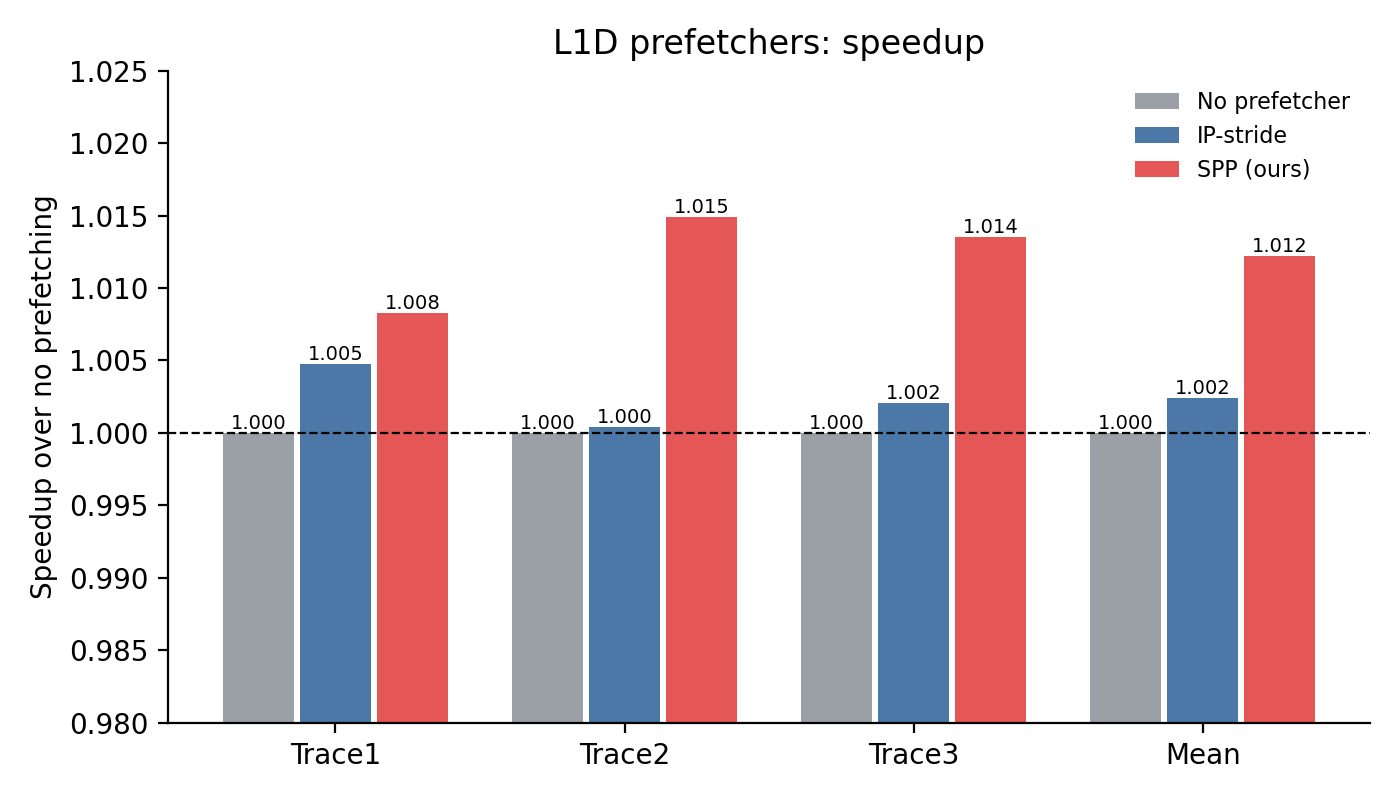
\includegraphics[width=.48\linewidth]{../results/task1/speedup.png}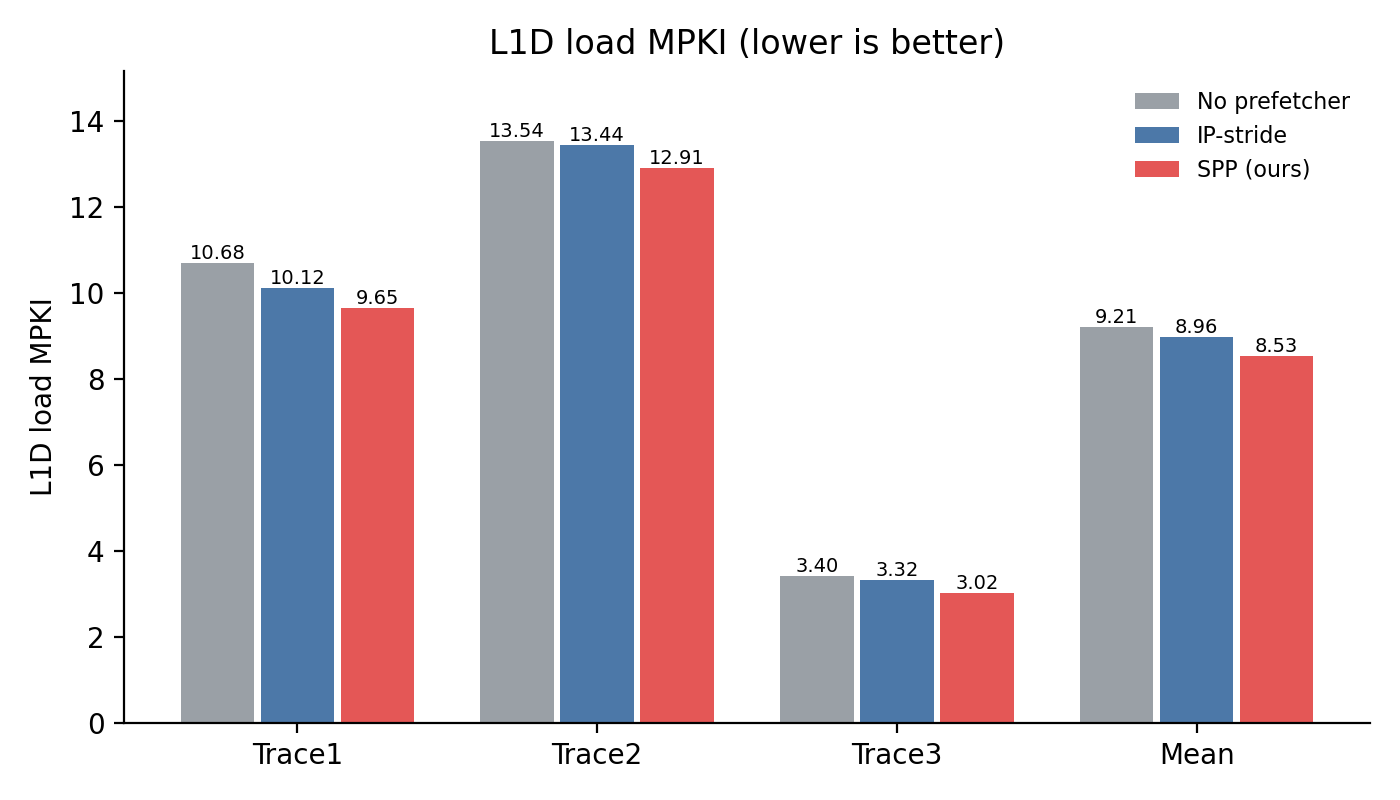
\includegraphics[width=.48\linewidth]{../results/task1/mpki.png}\\
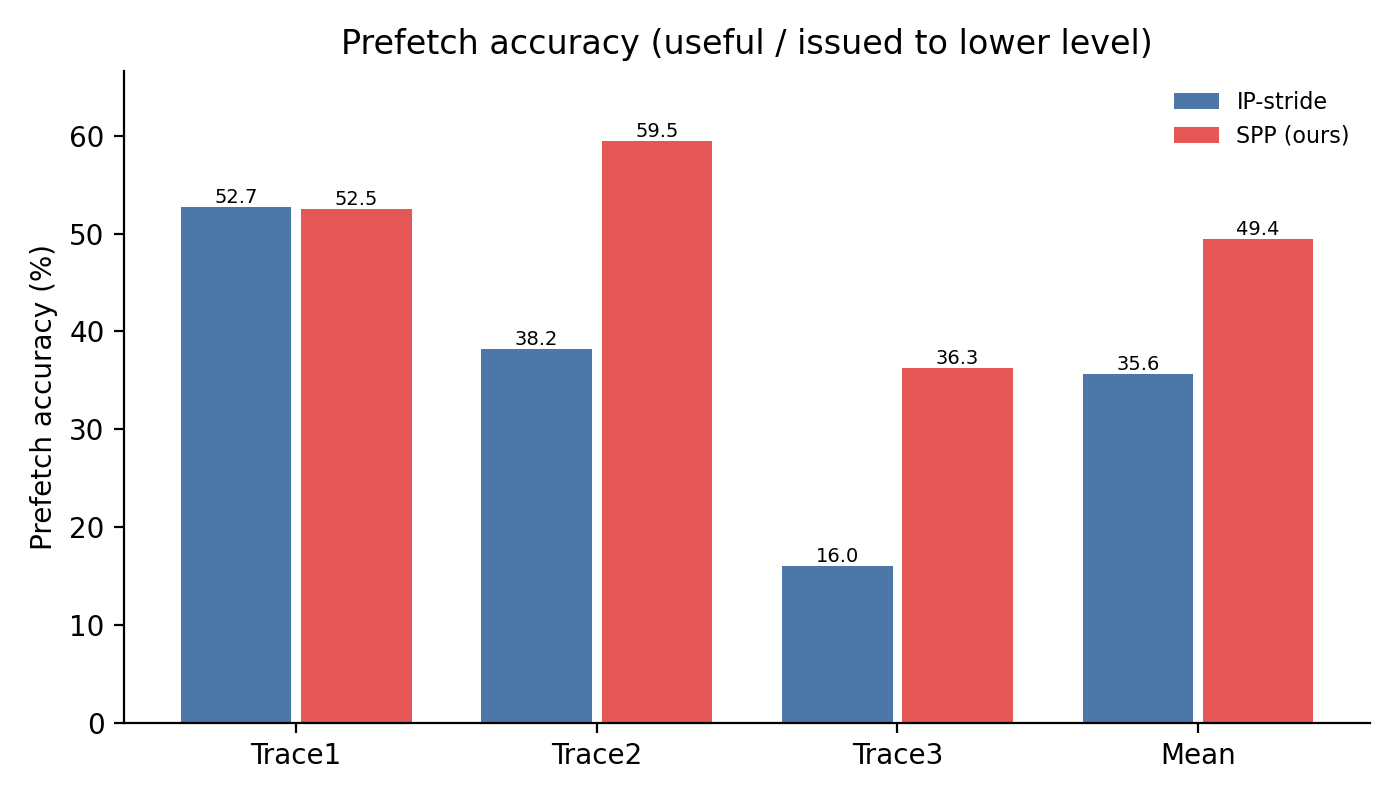
\includegraphics[width=.48\linewidth]{../results/task1/accuracy.png}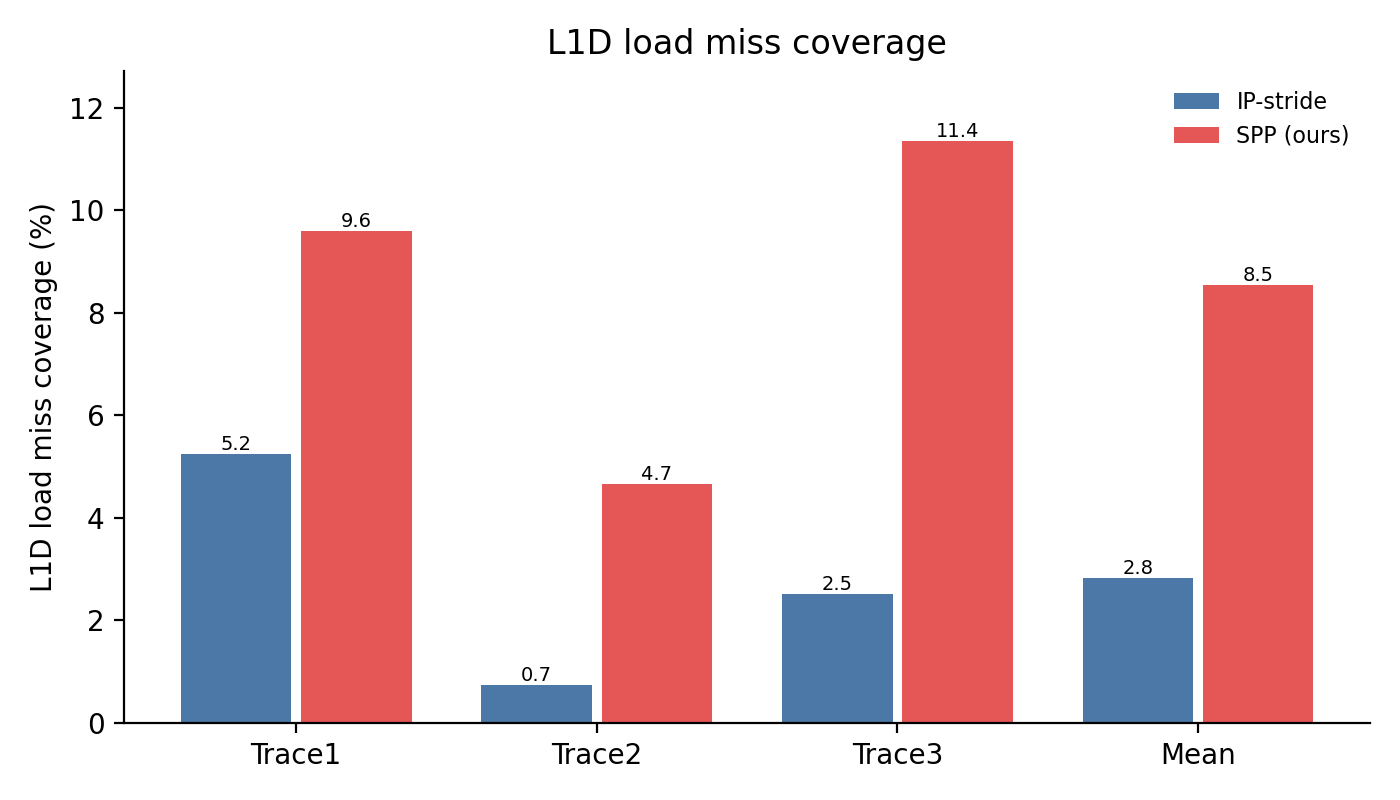
\includegraphics[width=.48\linewidth]{../results/task1/coverage.png}
\end{figure}
SPP beats IP-stride on every trace in both speedup and coverage. Its mean speedup is 1.0122 against 1.0024, and its mean coverage is 8.5\% against 2.8\%. Its accuracy is higher on Traces 2 and 3 and about the same on Trace 1 (52.5\% against 52.7\%). The absolute gains are small. A breakdown of the L1D misses showed that most of them come from IPs that are not in the table, from strides longer than a page (which the spec does not let us prefetch across) or from irregular accesses. Only about 3 to 5\% of the misses happen while a stride pattern is active.

\section*{Storage overhead (exact)}
\begin{tabular}{llp{9cm}r}\toprule
Structure & Entries & Bits per entry & Total bits\\\midrule
IP table & 256 & valid 1 + tag 8 + last line 16 + last stride 7 + uni conf 2 + 3$\times$7 signature + hist count 2 = 57 & 14592\\
Pattern table & 256 & stride 7 + conf 2 = 9 & 2304\\
Fallback table & 64 & stride 7 + conf 2 = 9 & 576\\
Recent-prefetch filter & 64 & valid 1 + tag 10 = 11 & 704\\
Counters & n/a & issued 9 + useful 9 + degree 3 & 21\\\midrule
\textbf{Total} & & 2274.6 B $\approx$ 2.2 KB & \textbf{18197}\\\bottomrule
\end{tabular}

For comparison, the IP-stride prefetcher as coded uses 24 $\times$ (64+64+64+32) = 5376 bits, so SPP needs about 3.4$\times$ more storage.

\section*{Threshold and degree rationale}
The 75/50/25\% thresholds split accuracy into four bands. Above 75\%, almost every prefetch gets used, so a deep degree of 6 costs little. Between 50 and 75\% is the normal range, and we use 4. Between 25 and 50\%, more than half of the prefetches are wasted, so the degree drops to 2. Below 25\%, prefetching costs more in bandwidth and L1D pollution than it gains, so only one line is fetched. These are simply the quartile boundaries, and we checked them with a sweep. Thresholds of 50/30/10, 60/40/20 and 90/70/40, and degree sets (8,4,2,1) and (8,6,4,2), all land within $\pm$0.1\% of the mean speedup (1.0115 to 1.0129), so the result is not sensitive to these choices. On an earlier version of the design without the fallback table, fixed degrees of 1, 2, 4 and 6 gave mean speedups of 1.0076, 1.0091, 1.0101 and 1.0102, so going deeper helps up to 4 and then flattens out. On the final design, dynamic throttling gives the same speedup as a fixed degree of 4 (1.0122 against 1.0124) but with 4 to 9 points higher accuracy. In other words, it saves bandwidth without losing performance.

\section*{Ablations and design validation}
\begin{tabular}{lcc}\toprule Configuration & Mean speedup & Note\\\midrule
Uniform stride only (no pattern table) & 1.0043 & $\approx$ IP-stride-like\\
Pattern table, no fallback & 1.0100 & \\
Pattern table + fallback (final) & 1.0122 & \\\bottomrule\end{tabular}

We also varied the IP-table size without the fallback table. 64, 128, 256, 512 and 1024 entries gave 1.0054, 1.0078, 1.0100, 1.0107 and 1.0111 (6.7, 10.3, 17.6, 32.2 and 61.4 Kbit), and we picked 256 entries as the knee of this curve. A single table indexed by the last 2 strides reached 1.0126, which is within noise of the final hybrid. We kept the hybrid because a 3-stride signature can tell longer patterns apart. On synthetic tests (uniform, non-uniform, phase changes, random and interleaved IPs), SPP covers about 97\% of the misses on regular streams and about 0\% on random ones, with no page-boundary violations in 186K prefetches. Its one weak spot is several interleaved IPs that share a signature in the pattern table (78\% coverage). Mixing IP bits into the index would help there, but it lowered the speedup on the real traces, so we left it out.

\section*{Task 2A: Instruction-conscious L2 replacement (I-RRIP)}
All Task 2 runs use no L1D prefetcher, so the replacement policy is evaluated on its own (Task 3 combines it with SPP). The baseline is LRU at L2.

{\sloppy \textbf{Exposing instruction information.} We added a 9th parameter, \texttt{isInstruction}, to \texttt{update\_replacement\_state} for every cache. This touched the declarations in \texttt{inc/cache.h} and every \texttt{replacement/*\_repl} file. The six call sites in \texttt{src/cache.cc} pass the packet's \texttt{instruction} field (from the MSHR entry on a fill, and from the RQ, WQ or PQ entry on a hit). The BTB calls in \texttt{src/ooo\_cpu.cc} pass 0. For eviction, the policy reads each line's \texttt{BLOCK::instruction} bit through the \texttt{current\_set} argument of \texttt{find\_victim}. \texttt{fill\_cache} already sets this bit for L2C lines filled by instruction loads and prefetches.\par}

\textbf{Policy} (\texttt{replacement/irrip.l2c\_repl}, with a 2-bit RRPV as in SRRIP):
\begin{itemize}[nosep]
\item \textbf{Insertion:} instruction lines at RRPV 1, data lines at RRPV 3 (SRRIP: both at 2).
\item \textbf{Promotion:} an instruction hit sets RRPV to 0, and a data hit lowers it by 1 (SRRIP: both go to 0).
\item \textbf{Eviction:} among the lines at RRPV 3, a data line is evicted before an instruction line. Aging is unchanged.
\end{itemize}

\textbf{Results} (25M warmup + 25M simulation instructions, speedup is the geometric mean over the three traces).
\textbf{IPC}\\[2pt]
\begin{tabular}{lrrrr}\toprule
Config & Trace1 & Trace2 & Trace3 & Mean \\ \midrule
Baseline (LRU) & 0.2322 & 0.2513 & 0.3819 & 0.2885 \\
SRRIP & 0.2322 & 0.2518 & 0.3816 & 0.2885 \\
I-RRIP & 0.2319 & 0.2597 & 0.3826 & 0.2914 \\
\bottomrule\end{tabular}
\medskip

\textbf{Speedup over baseline}\\[2pt]
\begin{tabular}{lrrrr}\toprule
Config & Trace1 & Trace2 & Trace3 & Mean \\ \midrule
Baseline (LRU) & 1.0000 & 1.0000 & 1.0000 & 1.0000 \\
SRRIP & 0.9999 & 1.0022 & 0.9993 & 1.0004 \\
I-RRIP & 0.9986 & 1.0334 & 1.0020 & 1.0112 \\
\bottomrule\end{tabular}
\medskip

\textbf{L2C load MPKI}\\[2pt]
\begin{tabular}{lrrrr}\toprule
Config & Trace1 & Trace2 & Trace3 & Mean \\ \midrule
Baseline (LRU) & 17.703 & 27.560 & 3.960 & 16.408 \\
SRRIP & 17.619 & 26.012 & 4.037 & 15.889 \\
I-RRIP & 18.578 & 20.104 & 3.928 & 14.204 \\
\bottomrule\end{tabular}
\medskip

\textbf{L2C instruction load MPKI}\\[2pt]
\begin{tabular}{lrrrr}\toprule
Config & Trace1 & Trace2 & Trace3 & Mean \\ \midrule
Baseline (LRU) & 10.368 & 18.892 & 1.124 & 10.128 \\
SRRIP & 10.563 & 17.980 & 1.190 & 9.911 \\
I-RRIP & 9.316 & 9.435 & 0.811 & 6.520 \\
\bottomrule\end{tabular}
\medskip

\textbf{L2C data load MPKI}\\[2pt]
\begin{tabular}{lrrrr}\toprule
Config & Trace1 & Trace2 & Trace3 & Mean \\ \midrule
Baseline (LRU) & 7.334 & 8.668 & 2.837 & 6.280 \\
SRRIP & 7.056 & 8.032 & 2.846 & 5.978 \\
I-RRIP & 9.263 & 10.669 & 3.118 & 7.683 \\
\bottomrule\end{tabular}
\medskip

\begin{figure}[H]\centering
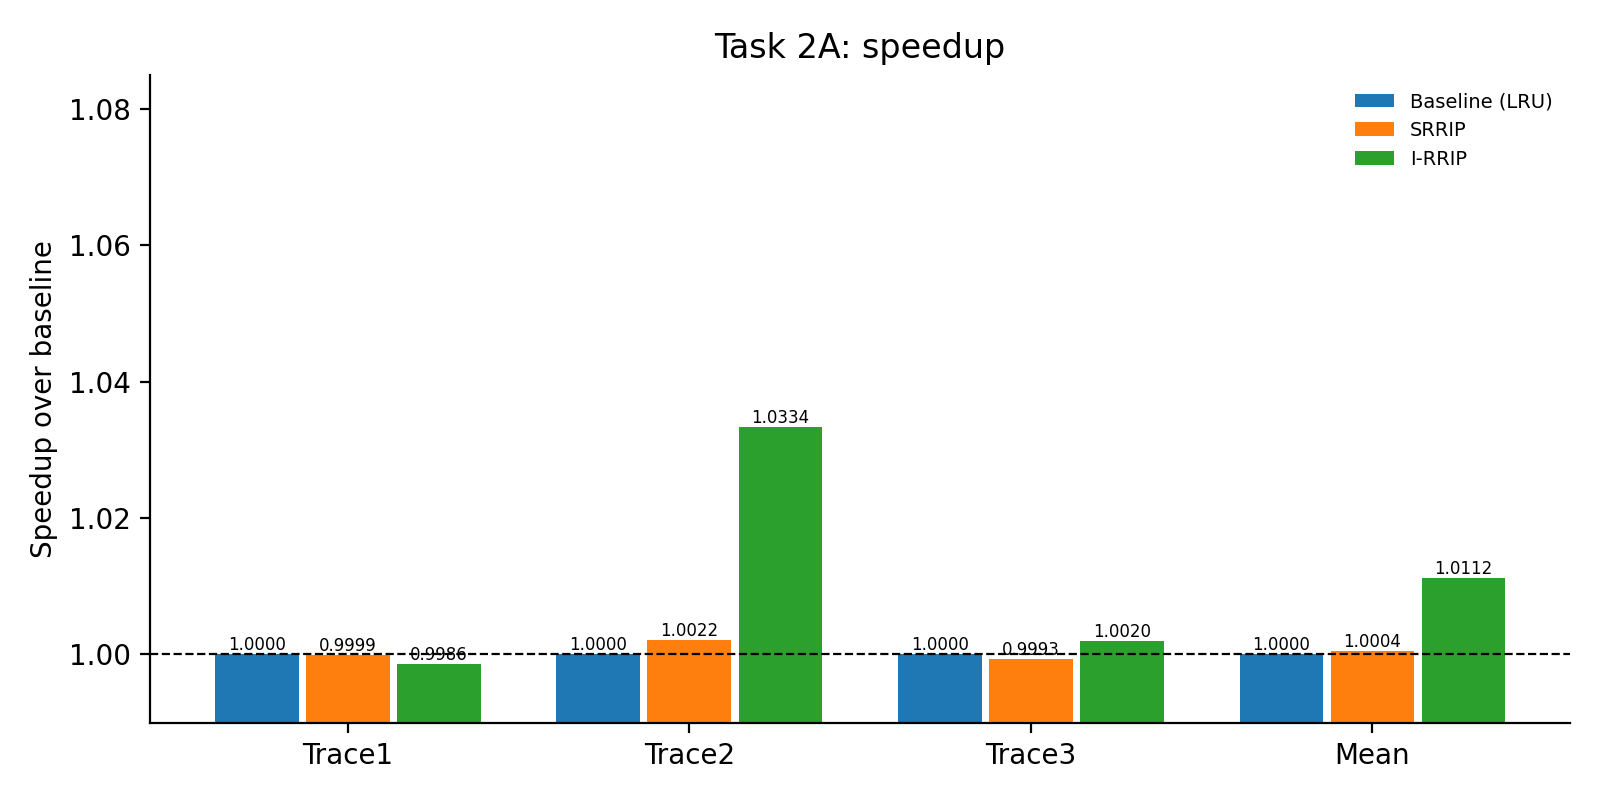
\includegraphics[width=.48\linewidth]{../results/task2a/speedup.png}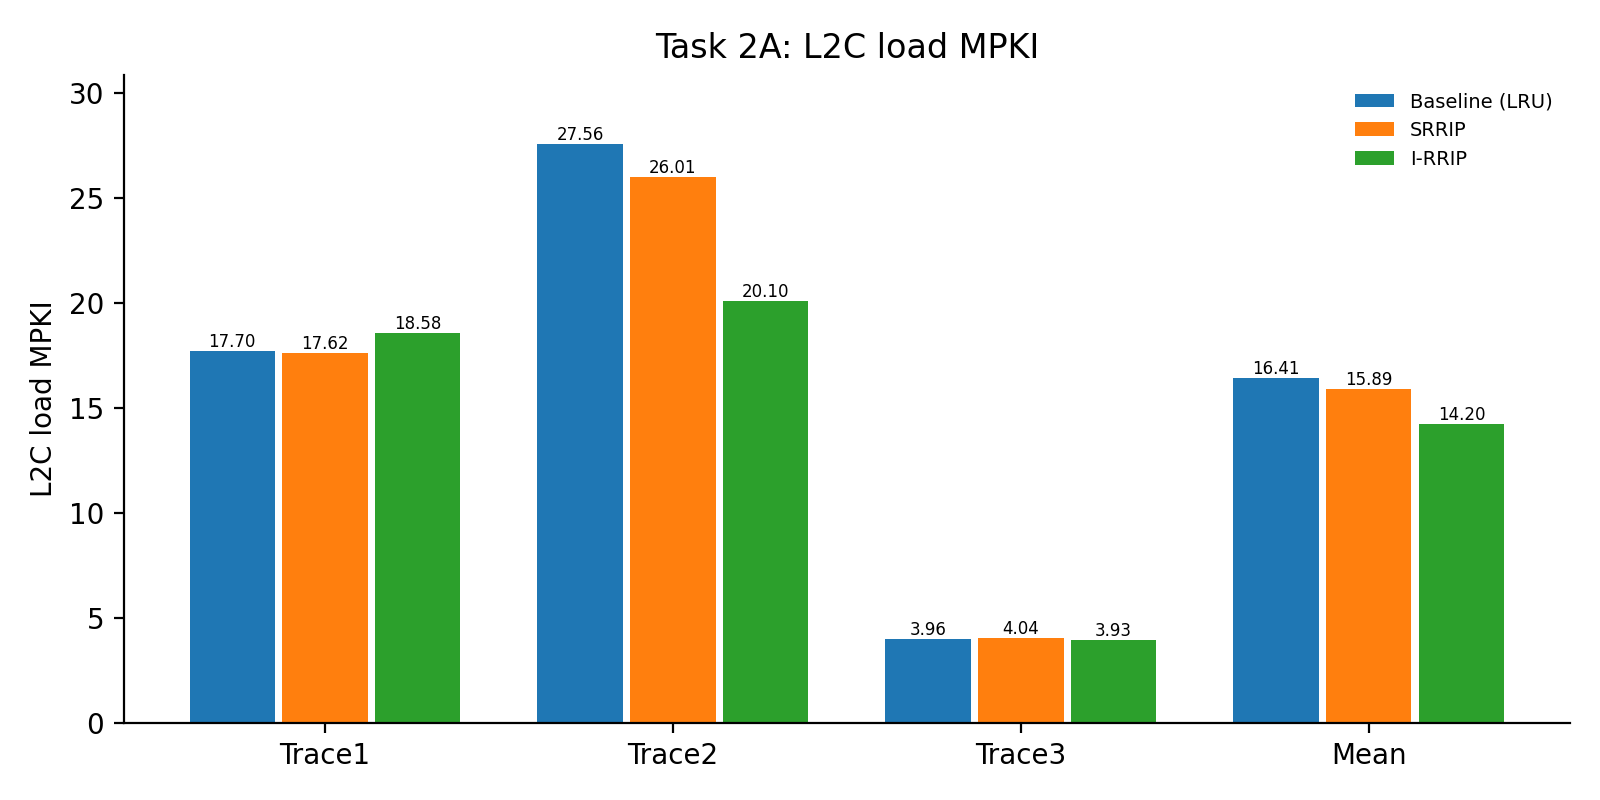
\includegraphics[width=.48\linewidth]{../results/task2a/l2_mpki.png}\\
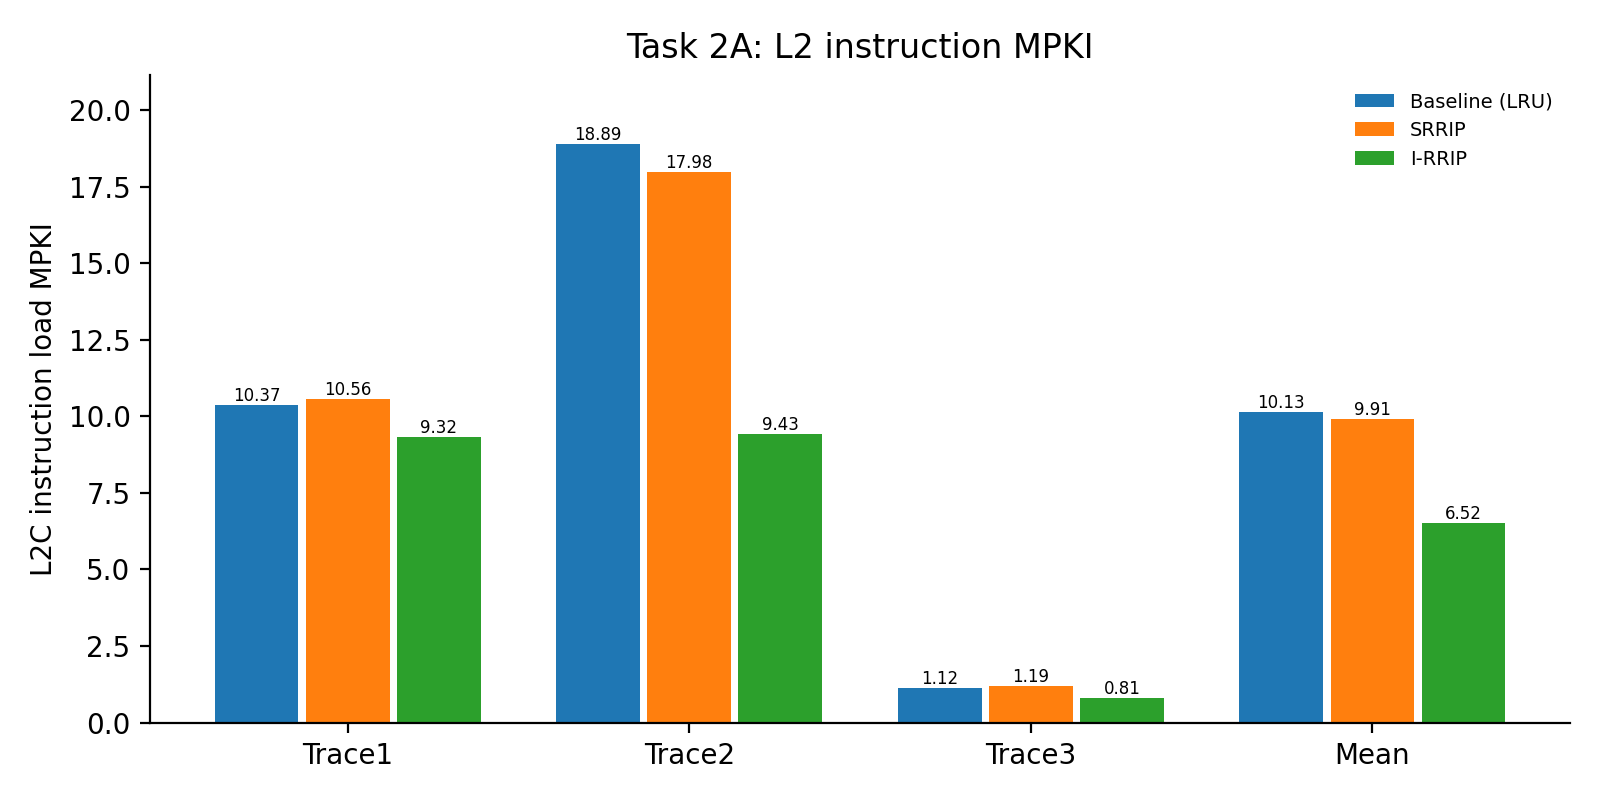
\includegraphics[width=.48\linewidth]{../results/task2a/l2_instr_mpki.png}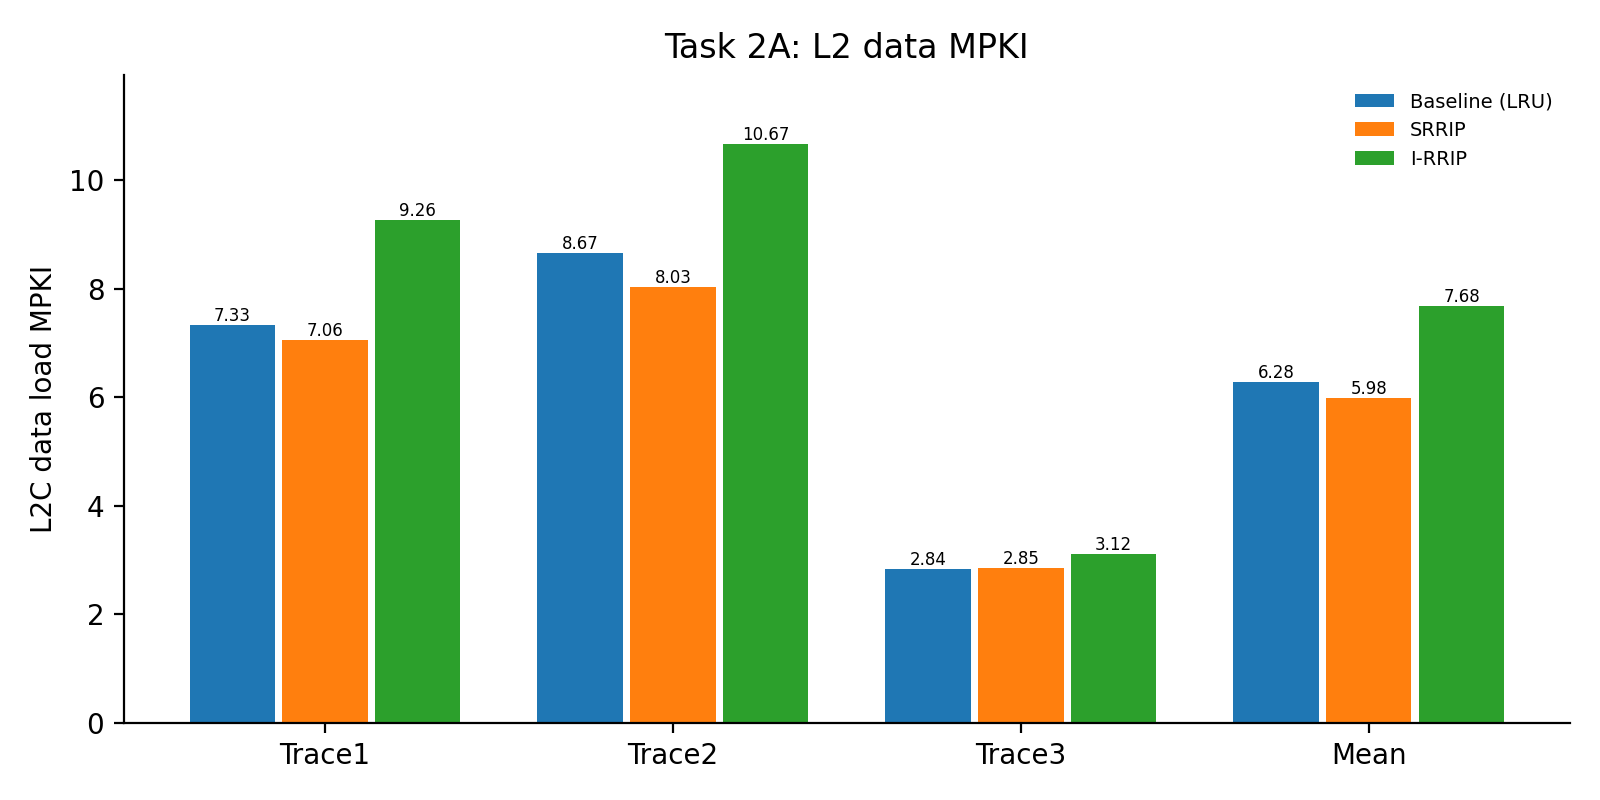
\includegraphics[width=.48\linewidth]{../results/task2a/l2_data_mpki.png}
\end{figure}
\textbf{Findings.} I-RRIP reaches a mean speedup of 1.0112, against 1.0004 for SRRIP. It cuts the mean L2 instruction load MPKI from 9.91 (SRRIP) to 6.52, a 34\% drop. The price is a higher data load MPKI, which rises from 5.98 to 7.68 ($+$28\%). Total L2 load MPKI still falls by 11\% (15.89 to 14.20). Instruction misses are both the larger share and the more expensive ones: an instruction miss stalls the front end, while out-of-order execution hides part of a data miss. Most of the gain comes from Trace 2, which has by far the highest L2 instruction MPKI. There, instruction MPKI almost halves (17.98 to 9.43) and IPC goes up 3.3\% over the LRU baseline. Trace 3 gains 0.2\%. Trace 1 loses 0.14\%. Its LLC misses on 66 to 70\% of the loads it receives under every policy, so the extra L2 data misses mostly go all the way to DRAM, and they outnumber the instruction misses saved (data MPKI $+$2.21 against instruction MPKI $-$1.25, compared with SRRIP). Blindly prioritising instructions is therefore not always the right call, and this is what motivates Task 2B.

{\sloppy\textbf{How the design was chosen.} We made every part of the policy a compile-time knob: instruction insertion RRPV (0, 1 or 2), data insertion (RRPV 2, RRPV 3, or bimodal, which is RRPV 3 with every 32nd insertion at 2), instruction promotion (to 0 or decrement), data promotion (to 0, decrement or unchanged), and two eviction options (prefer a data victim among the RRPV-3 lines, and age data lines by 2 instead of 1). The full grid has $3\cdot3\cdot2\cdot3\cdot2\cdot2 = 216$ configurations, so we searched it in two stages. \emph{Stage 1} (14 configurations) turned on one change at a time. We did this both on top of SRRIP, which gives an ablation of insertion, promotion and eviction, and on top of I+P. I+P is the combination of instruction insertion at RRPV 0 (with instruction hits going to 0) and data decrement on a hit. With every knob at its SRRIP value, the knob file reproduces \texttt{rrip.l2c\_repl} exactly, which validates the knob implementation.\par}

\smallskip\noindent\begin{minipage}{\linewidth}\textbf{Stage 1: speedup over baseline}\\[2pt]
\begin{tabular}{lrrrr}\toprule
Configuration & Trace1 & Trace2 & Trace3 & Mean \\ \midrule
SRRIP (all knobs off) & 0.9999 & 1.0022 & 0.9993 & 1.0004 \\
Insertion only (instr RRPV 0) & 1.0000 & 1.0130 & 0.9999 & 1.0043 \\
Promotion only (data decrement) & 1.0008 & 1.0085 & 0.9995 & 1.0029 \\
Eviction only (prefer data) & 0.9998 & 1.0185 & 0.9993 & 1.0058 \\
Eviction only (age data faster) & 1.0004 & 1.0088 & 0.9994 & 1.0029 \\
Insertion + promotion (I+P) & 0.9998 & 1.0176 & 0.9999 & 1.0058 \\
I+P + prefer data & 0.9994 & 1.0229 & 1.0000 & 1.0074 \\
I+P + age data faster & 0.9993 & 1.0196 & 1.0001 & 1.0063 \\
I+P + both eviction options & 0.9983 & 1.0251 & 1.0000 & 1.0077 \\
I+P, instr insert RRPV 1 & 1.0003 & 1.0154 & 0.9999 & 1.0052 \\
I+P, data insert RRPV 3 & 0.9968 & 1.0291 & 1.0013 & 1.0089 \\
I+P, data insert bimodal & 0.9971 & 1.0283 & 1.0008 & 1.0087 \\
I+P, data not promoted & 0.9978 & 1.0202 & 1.0000 & 1.0059 \\
I+P, instr decrement on hit & 1.0001 & 1.0176 & 1.0001 & 1.0059 \\
\bottomrule\end{tabular}
\end{minipage}
\begin{figure}[H]\centering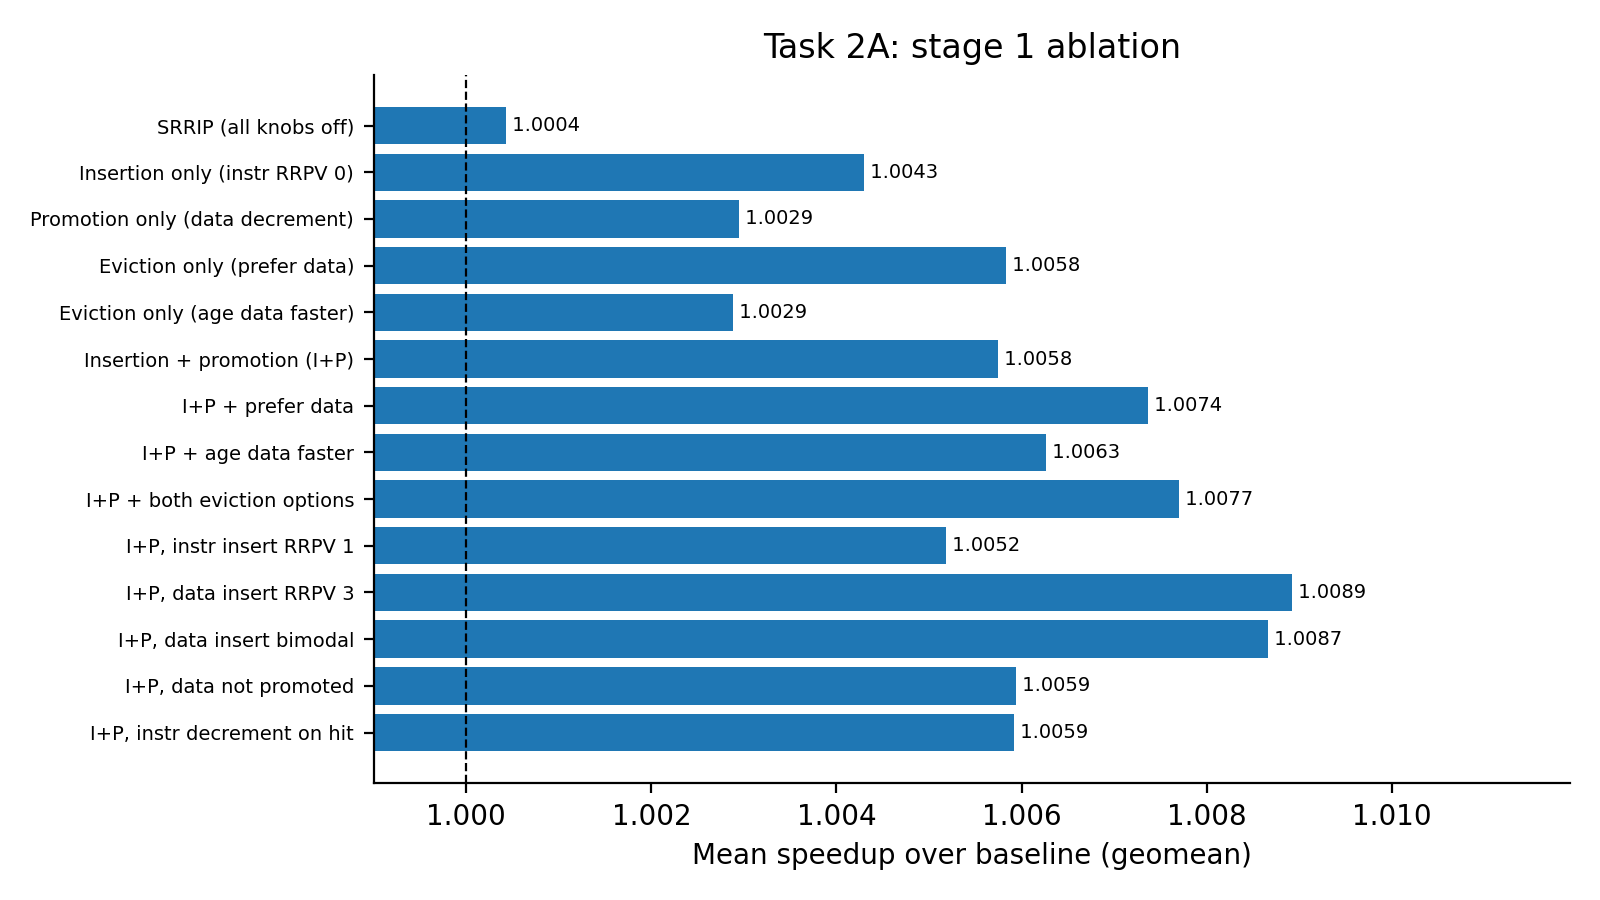
\includegraphics[width=.7\linewidth]{../results/task2a/ablation_stage1.png}\end{figure}
\emph{Stage 2} took the knobs that moved the mean speedup by at least 0.05\% in stage 1, which were instruction insertion, data insertion and both eviction options. Each was tested at its two best values in a full factorial ($2^4 = 16$ configurations). Promotion was fixed at instruction-to-0 and data-decrement. The two instruction options tied within 0.01\%, sending data to 0 was clearly worse, and leaving data unpromoted tied with decrement but is unsafe once data is inserted at RRPV 3 (explained below). Two stage-2 points repeat stage-1 points and reproduced bit-exactly.

\smallskip\noindent\begin{minipage}{\linewidth}\textbf{Stage 2: speedup over baseline}\\[2pt]
\begin{tabular}{lrrrr}\toprule
Instr insert / data insert / prefer data / age data & Trace1 & Trace2 & Trace3 & Mean \\ \midrule
instr 1 / data RRPV 3 / prefer on / age on & 0.9974 & 1.0348 & 1.0020 & 1.0113 \\
instr 1 / data RRPV 3 / prefer on / age off (chosen) & 0.9986 & 1.0334 & 1.0020 & 1.0112 \\
instr 1 / data bimodal / prefer on / age on & 0.9980 & 1.0343 & 1.0015 & 1.0111 \\
instr 1 / data RRPV 3 / prefer off / age on & 0.9982 & 1.0337 & 1.0018 & 1.0111 \\
instr 1 / data bimodal / prefer on / age off & 0.9990 & 1.0332 & 1.0014 & 1.0111 \\
instr 1 / data bimodal / prefer off / age on & 0.9986 & 1.0327 & 1.0012 & 1.0107 \\
instr 1 / data RRPV 3 / prefer off / age off & 0.9993 & 1.0313 & 1.0017 & 1.0107 \\
instr 1 / data bimodal / prefer off / age off & 0.9998 & 1.0305 & 1.0012 & 1.0104 \\
instr 0 / data RRPV 3 / prefer on / age off & 0.9961 & 1.0300 & 1.0014 & 1.0091 \\
instr 0 / data RRPV 3 / prefer off / age off & 0.9968 & 1.0291 & 1.0013 & 1.0089 \\
instr 0 / data bimodal / prefer on / age on & 0.9954 & 1.0299 & 1.0011 & 1.0087 \\
instr 0 / data bimodal / prefer off / age on & 0.9963 & 1.0291 & 1.0011 & 1.0087 \\
instr 0 / data bimodal / prefer on / age off & 0.9964 & 1.0290 & 1.0010 & 1.0087 \\
instr 0 / data bimodal / prefer off / age off & 0.9971 & 1.0283 & 1.0008 & 1.0087 \\
instr 0 / data RRPV 3 / prefer off / age on & 0.9955 & 1.0297 & 1.0011 & 1.0087 \\
instr 0 / data RRPV 3 / prefer on / age on & 0.9946 & 1.0300 & 1.0014 & 1.0085 \\
\bottomrule\end{tabular}
\end{minipage}

\medskip
\textbf{Rationale: insertion (modified).} Insertion decides how long a new line gets to prove itself, so it is the most direct way to favour instructions. Code lines are reused across loop iterations and repeated calls, but often at reuse distances larger than the L1I can hold. Inserting data at RRPV 3 makes a new data line the first candidate for eviction unless it gets reused. On top of I+P this was the biggest single improvement (1.0058 to 1.0089), which suggests that most data lines reaching L2 in these traces are not reused before they would be evicted anyway. Instructions go in at RRPV 1 rather than 0, and only the full factorial showed this. With data inserted at RRPV 2, instruction RRPV 0 was slightly better (1.0058 against 1.0052). Once data is inserted at RRPV 3, though, RRPV 1 wins in all eight pairings, by 0.17 to 0.27\%. Data at RRPV 3 already gives code a two-step head start, so RRPV 0 is no longer needed to protect code from data. All it does is let code that runs only once (cold paths, one-time initialisation) push out code that is actually reused. Bimodal data insertion came within about 0.04\% of RRPV 3 in every stage-2 pairing. It was slightly ahead in two of them, by at most 0.02\%, but it needs an extra counter, so we kept plain RRPV 3.

\textbf{Rationale: promotion (modified for data only).} An instruction hit is strong evidence of a hot code path, so instructions keep SRRIP's promote-to-0 rule. Decrementing instead gave the same result (1.0059 against 1.0058), so we kept the simpler, standard rule. Data uses frequency-based promotion: each hit moves the line one step closer, so only data that is reused again and again earns the protection that code gets on its first hit. Promoting data straight to 0 would undo the insertion bias after a single reuse, and it lowered the mean speedup from 1.0058 to 1.0043 compared with decrementing. Leaving data unpromoted tied with decrement on its own (1.0059). Combined with insertion at RRPV 3, however, a reused data line would never leave the eviction position, so decrement is the safe choice.

\textbf{Rationale: eviction (modified as a tie-breaker only).} SRRIP evicts the first line it finds at RRPV 3. Preferring a data line among those candidates costs nothing extra, because the instruction bit is already stored with every line. It only matters when code and data are equally old, and in that case evicting the data line fits the rest of the policy. On its own, it gave the largest gain of any single change on top of SRRIP (1.0004 to 1.0058), and in stage 2 it added about 0.05\%. We did \emph{not} adopt faster data aging. On top of the chosen insertion and promotion it changed the mean speedup by only 0.01\% (1.0112 against 1.0113), but it raised the Trace 1 loss from 0.14\% to 0.26\% and needs a second aging rule. Aging is therefore left as in SRRIP.

\textbf{Storage.} Each line needs a 2-bit RRPV (as in SRRIP) and 1 instruction bit, which ChampSim's L2C already keeps in \texttt{BLOCK}. For 1024 sets $\times$ 8 ways, that is 16384 + 8192 = 24576 bits (3 KB). Only the 8192 instruction bits (1 KB) are extra compared with SRRIP, and no counters or tables are added.

\section*{Task 2B: Dynamic I-RRIP}
Same setup as Task 2A (no L1D prefetcher, LRU baseline, 25M warmup + 25M simulation instructions).

{\sloppy \textbf{Policy.} \texttt{replacement/dyn\_irrip.l2c\_repl} uses set dueling between SRRIP and I-RRIP. The prefetch rules added in Task 3 never trigger here, because no prefetcher is used.\par}
\begin{itemize}[nosep]
\item \textbf{Leader sets:} 32 sets always run SRRIP and 32 always run I-RRIP, which is 64 of the 1024 sets (6.25\%). The cache is split into 32 regions of 32 sets. In region $r$, the set at offset $r$ is the SRRIP leader and the set at offset $31-r$ (the complement) is the I-RRIP leader. Both groups are therefore spread over the whole cache and never overlap. Spotting a leader takes a 5-bit compare on the set index, with no table.
\item \textbf{Selector:} a 10-bit saturating counter PSEL, initialised to 512. A demand load miss in an SRRIP leader increments it, and one in an I-RRIP leader decrements it. The follower sets (the other 960) run I-RRIP when the MSB of PSEL is 1 (the SRRIP leaders are missing more) and SRRIP otherwise.
\item \textbf{SRRIP mode:} insert at RRPV 2, promote to 0 on a hit, evict the first line at RRPV 3.
\item \textbf{I-RRIP mode:} instruction lines are inserted at RRPV 1 and promoted to 0 on a hit. Data lines are inserted at RRPV 3 and decremented by 1 on a hit. Among lines at RRPV 3, a data line is evicted first. When no line is at RRPV 3, data lines age by 2 and instruction lines by 1.
\end{itemize}

\textbf{Results.} ``I-RRIP mode, static'' is the I-RRIP mode above run on every set. It separates the effect of the selector from the effect of the mode itself.
\textbf{IPC}\\[2pt]
\begin{tabular}{lrrrr}\toprule
Config & Trace1 & Trace2 & Trace3 & Mean \\ \midrule
Baseline (LRU) & 0.2322 & 0.2513 & 0.3819 & 0.2885 \\
SRRIP & 0.2322 & 0.2518 & 0.3816 & 0.2885 \\
I-RRIP (Task 2A) & 0.2319 & 0.2597 & 0.3826 & 0.2914 \\
I-RRIP mode, static & 0.2317 & 0.2600 & 0.3826 & 0.2914 \\
Dynamic I-RRIP & 0.2321 & 0.2597 & 0.3825 & 0.2914 \\
\bottomrule\end{tabular}
\medskip

\textbf{Speedup over baseline}\\[2pt]
\begin{tabular}{lrrrr}\toprule
Config & Trace1 & Trace2 & Trace3 & Mean \\ \midrule
Baseline (LRU) & 1.0000 & 1.0000 & 1.0000 & 1.0000 \\
SRRIP & 0.9999 & 1.0022 & 0.9993 & 1.0004 \\
I-RRIP (Task 2A) & 0.9986 & 1.0334 & 1.0020 & 1.0112 \\
I-RRIP mode, static & 0.9974 & 1.0348 & 1.0020 & 1.0113 \\
Dynamic I-RRIP & 0.9993 & 1.0335 & 1.0017 & 1.0114 \\
\bottomrule\end{tabular}
\medskip

\textbf{L2C load MPKI}\\[2pt]
\begin{tabular}{lrrrr}\toprule
Config & Trace1 & Trace2 & Trace3 & Mean \\ \midrule
Baseline (LRU) & 17.703 & 27.560 & 3.960 & 16.408 \\
SRRIP & 17.619 & 26.012 & 4.037 & 15.889 \\
I-RRIP (Task 2A) & 18.578 & 20.104 & 3.928 & 14.204 \\
I-RRIP mode, static & 18.700 & 19.927 & 3.931 & 14.186 \\
Dynamic I-RRIP & 17.665 & 20.108 & 3.937 & 13.903 \\
\bottomrule\end{tabular}
\medskip

\textbf{L2C instruction load MPKI}\\[2pt]
\begin{tabular}{lrrrr}\toprule
Config & Trace1 & Trace2 & Trace3 & Mean \\ \midrule
Baseline (LRU) & 10.368 & 18.892 & 1.124 & 10.128 \\
SRRIP & 10.563 & 17.980 & 1.190 & 9.911 \\
I-RRIP (Task 2A) & 9.316 & 9.435 & 0.811 & 6.520 \\
I-RRIP mode, static & 9.242 & 9.029 & 0.792 & 6.354 \\
Dynamic I-RRIP & 10.528 & 9.296 & 0.804 & 6.876 \\
\bottomrule\end{tabular}
\medskip

\textbf{L2C data load MPKI}\\[2pt]
\begin{tabular}{lrrrr}\toprule
Config & Trace1 & Trace2 & Trace3 & Mean \\ \midrule
Baseline (LRU) & 7.334 & 8.668 & 2.837 & 6.280 \\
SRRIP & 7.056 & 8.032 & 2.846 & 5.978 \\
I-RRIP (Task 2A) & 9.263 & 10.669 & 3.118 & 7.683 \\
I-RRIP mode, static & 9.459 & 10.897 & 3.139 & 7.832 \\
Dynamic I-RRIP & 7.137 & 10.811 & 3.133 & 7.027 \\
\bottomrule\end{tabular}
\medskip

\begin{figure}[H]\centering
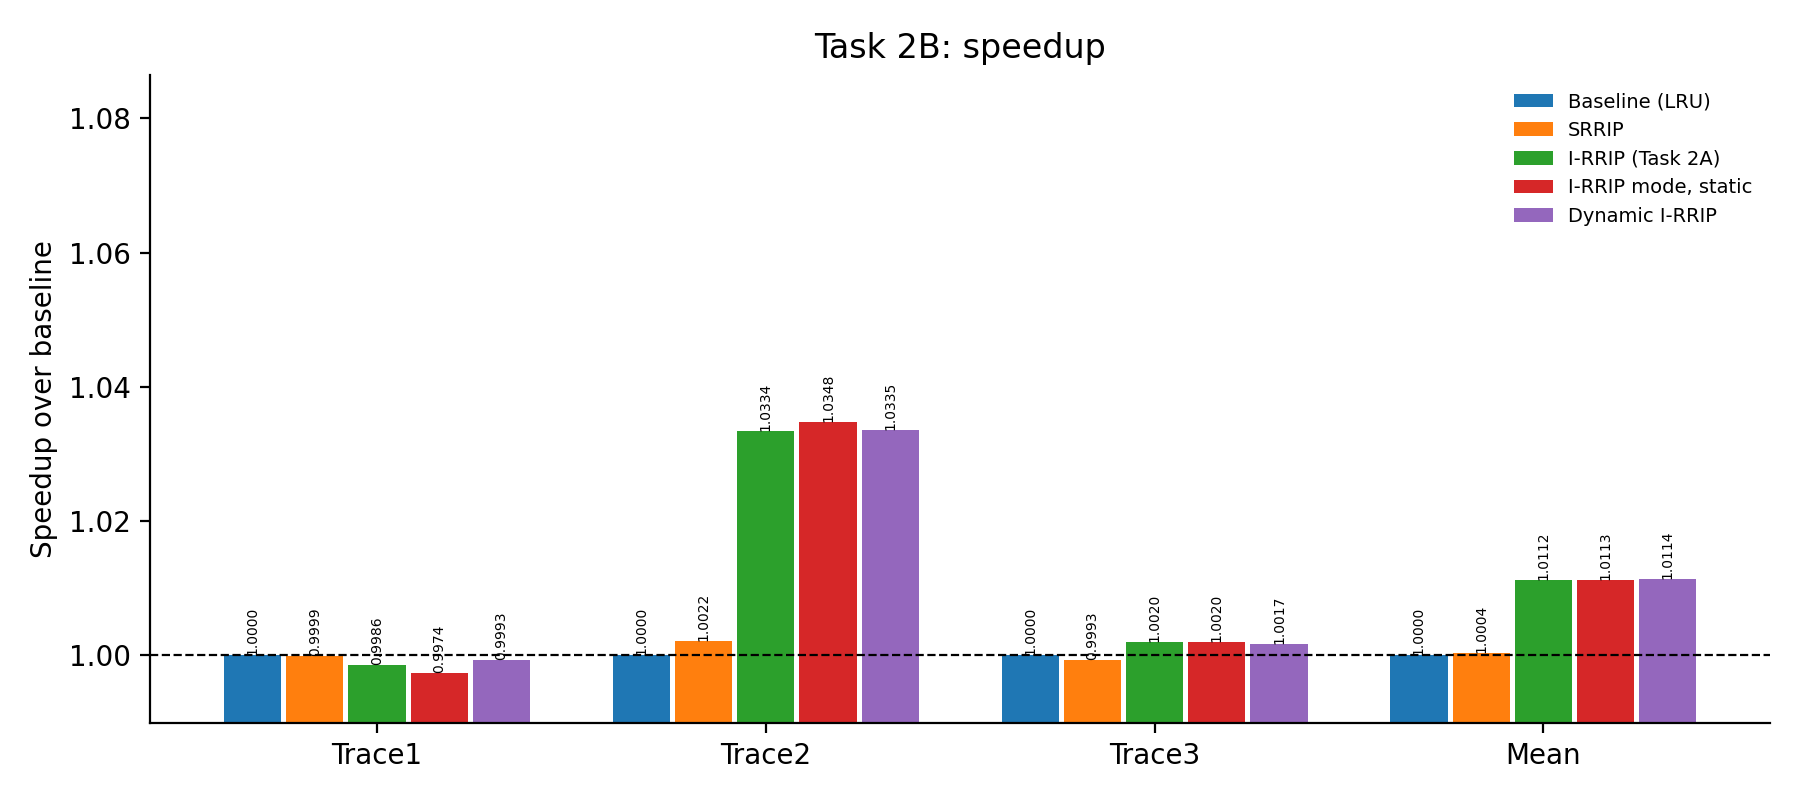
\includegraphics[width=.48\linewidth]{../results/task2b/speedup.png}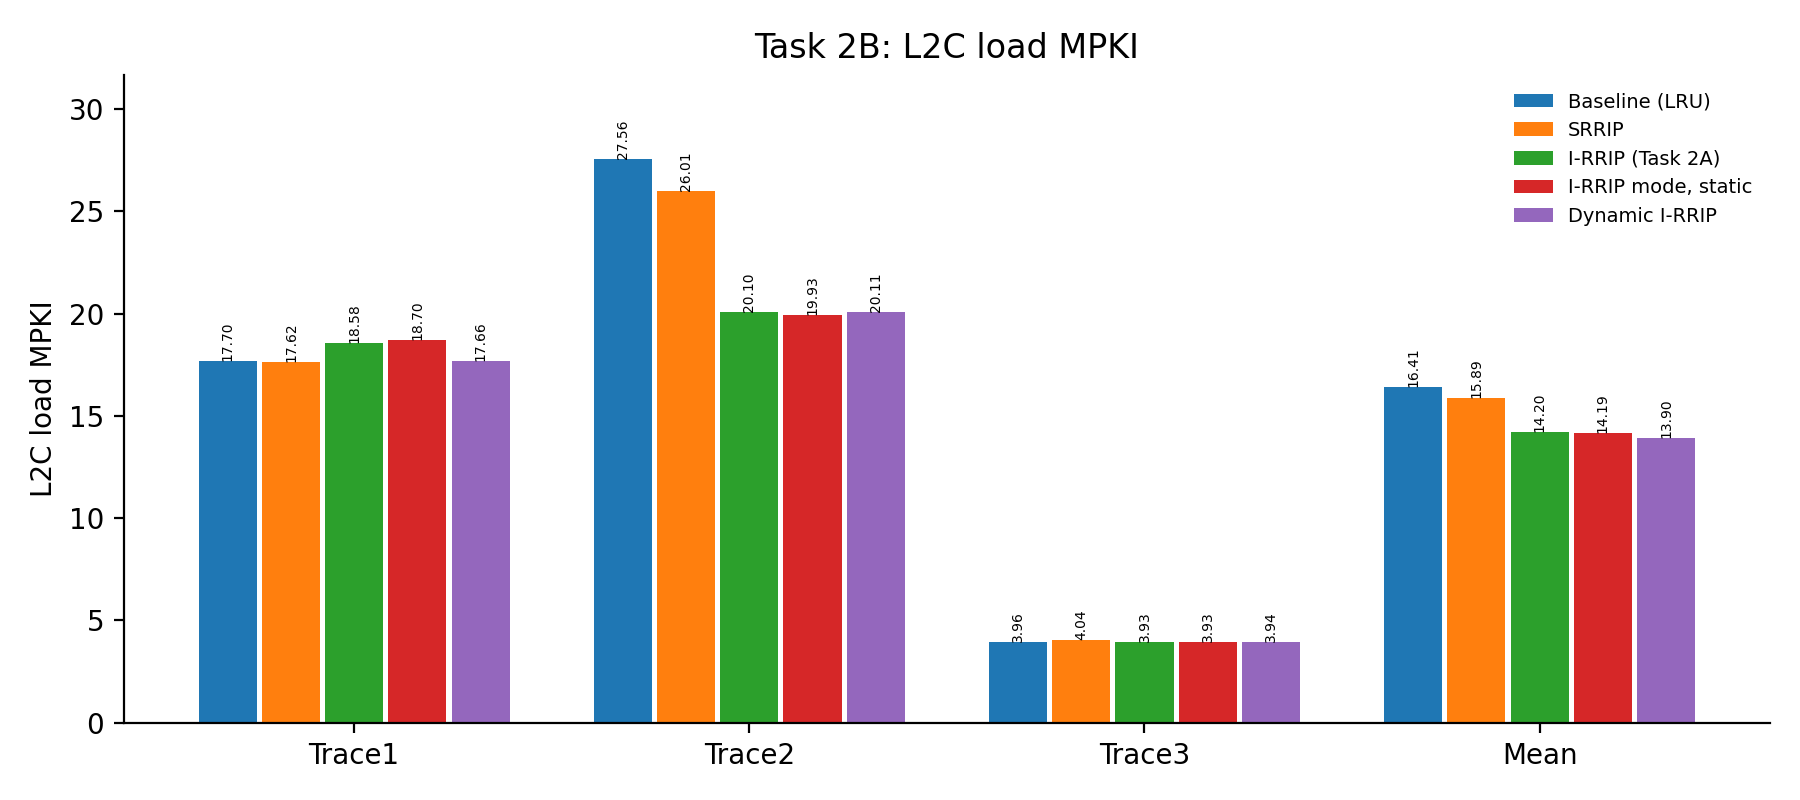
\includegraphics[width=.48\linewidth]{../results/task2b/l2_mpki.png}\\
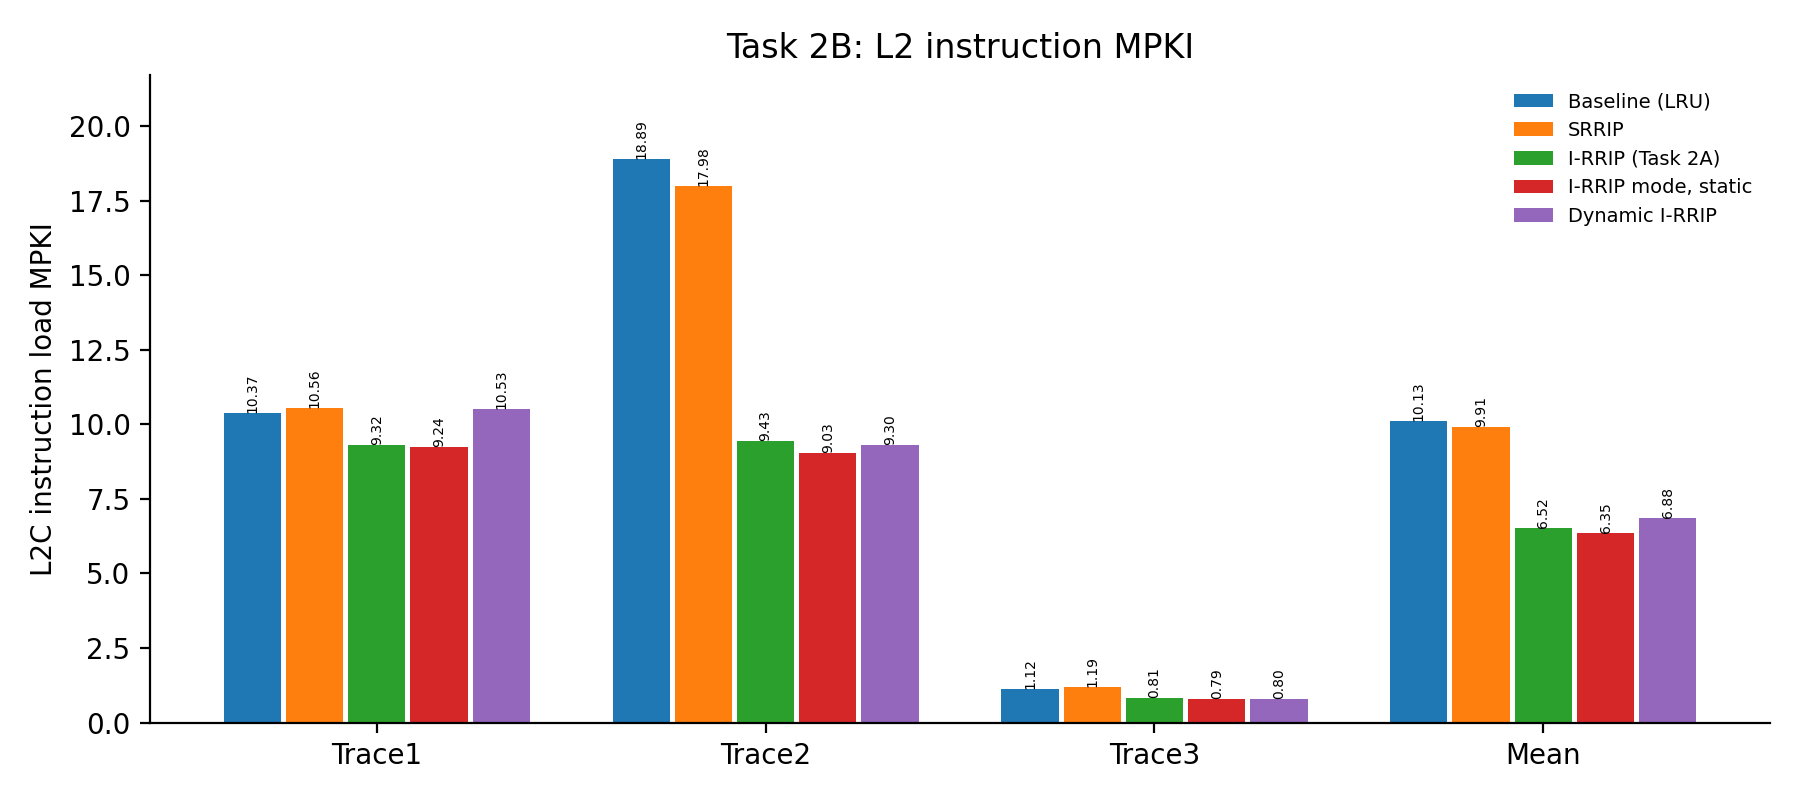
\includegraphics[width=.48\linewidth]{../results/task2b/l2_instr_mpki.png}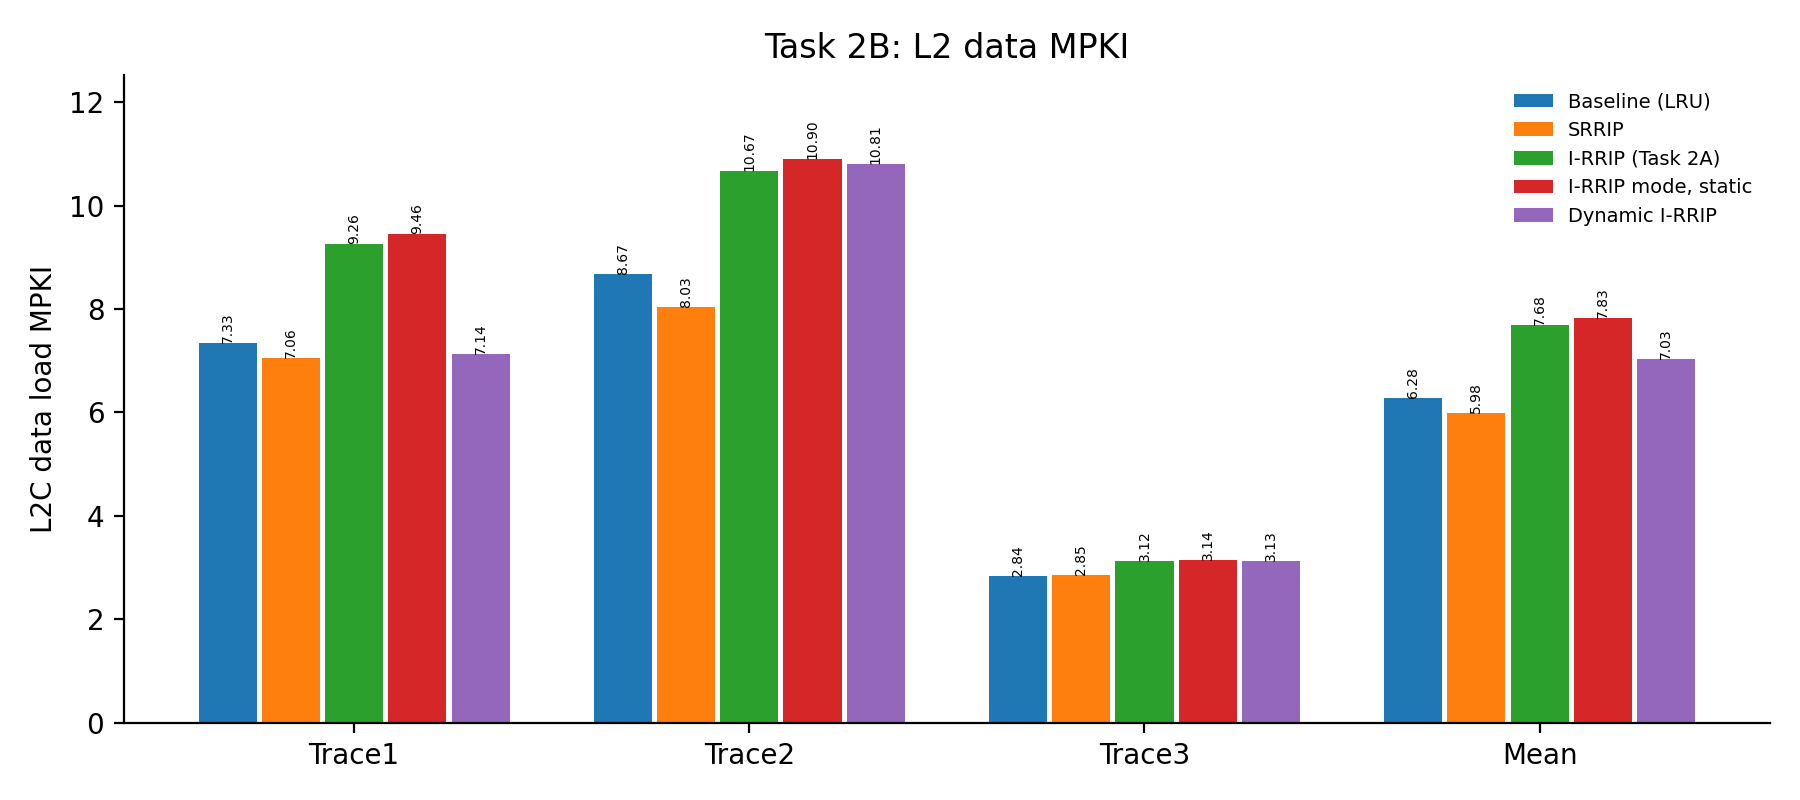
\includegraphics[width=.48\linewidth]{../results/task2b/l2_data_mpki.png}
\end{figure}
\smallskip\noindent\begin{minipage}{\linewidth}\textbf{Selector behaviour (after warmup)}\\[2pt]
\begin{tabular}{lrrrrr}\toprule
Trace & \multicolumn{2}{c}{Leader demand misses} & Final PSEL & Followers in & Mode \\
 & SRRIP & I-RRIP & (of 1023) & I-RRIP mode & switches \\ \midrule
Trace1 & 13403 & 15120 & 0 & 0.0\% & 0 \\
Trace2 & 19435 & 16414 & 1017 & 100.0\% & 0 \\
Trace3 & 3202 & 3006 & 1020 & 100.0\% & 0 \\
\bottomrule\end{tabular}
\end{minipage}

\medskip
\textbf{Findings.} The selector makes the right choice on every trace, and it never changes its mind after warmup. On Trace 1 the I-RRIP leaders miss 13\% more than the SRRIP leaders, PSEL stays at 0 and every follower set runs SRRIP. The Trace 1 loss shrinks from 0.26\% (static I-RRIP mode) to 0.07\%, and data MPKI goes back to the SRRIP level (7.14 against 7.06). On Traces 2 and 3 the SRRIP leaders miss more (18\% and 6.5\%), PSEL climbs close to 1023, and all followers run I-RRIP. Dynamic I-RRIP has the highest mean speedup of the policies in this table (1.0114) and the lowest mean L2 load MPKI (13.90, against 14.20 for Task 2A's I-RRIP and 15.89 for SRRIP). The best any selector between these two modes could do is pick the better static mode on each trace, which gives 1.0121. The remaining 0.07\% is the cost of the leader sets, which keep running the losing policy. On Trace 2, for example, the 32 SRRIP leaders lower the speedup from 1.0348 to 1.0335.

\textbf{Choice of the I-RRIP mode.} Task 2A and Task 2B use different I-RRIP settings, because the two tasks ask different questions. In Task 2A the policy is static, so whatever it does to a trace, that trace is stuck with it. We therefore chose it on all three traces and kept the setting without faster data aging. Its mean speedup is within noise of the best one (1.0112 against 1.0113), and it loses less on Trace 1 (0.14\% against 0.26\%).

In Task 2B, the I-RRIP rules are only one of two options, and set dueling falls back to SRRIP on a workload where they hurt. Trace 1 is such a workload. Replacement barely matters there (SRRIP is at 0.9999 against LRU), and every stage-2 I-RRIP setting was slightly below the baseline. So on Trace 1 the dynamic policy should pick SRRIP rather than a gentler I-RRIP, and the selector table shows that it does. The I-RRIP mode only needs to be strong on the workloads where it gets picked. Trace 2 is the case the problem statement describes: a large code footprint, with the highest L2 instruction MPKI under SRRIP (17.98). We therefore tuned the I-RRIP mode for Trace 2. Adding faster data aging raises Trace 2's speedup from 1.0334 to 1.0348 and cuts its instruction MPKI from 9.43 to 9.03. The cost is one extra aging rule, used only in sets running I-RRIP.

\textbf{How the design was chosen.} We made the number of leader sets, their placement and the PSEL width compile-time knobs. Two sanity runs force every follower set into one mode. They reproduce static SRRIP and the static I-RRIP mode to within 0.05\% on every trace (the small difference comes from the leader sets of the other policy), which confirms that the mode switch works.

\smallskip\noindent\begin{minipage}{\linewidth}\textbf{Sanity check: speedup over baseline}\\[2pt]
\begin{tabular}{lrrrr}\toprule
Configuration & Trace1 & Trace2 & Trace3 & Mean \\ \midrule
Followers forced to SRRIP & 0.9997 & 1.0025 & 0.9993 & 1.0005 \\
Static SRRIP & 0.9999 & 1.0022 & 0.9993 & 1.0004 \\
Followers forced to I-RRIP & 0.9975 & 1.0343 & 1.0019 & 1.0111 \\
Static I-RRIP mode & 0.9974 & 1.0348 & 1.0020 & 1.0113 \\
\bottomrule\end{tabular}
\end{minipage}

\medskip
The sensitivity study then ran the full grid of 8, 16 or 32 leader sets per policy, placed either contiguously (sets $0..N-1$ lead SRRIP and $N..2N-1$ lead I-RRIP) or spread as above, with an 8, 10 or 12-bit PSEL (18 configurations). The last column is the share of Trace 1 follower updates done in I-RRIP mode, and the right answer for Trace 1 is 0\%. On Trace 2 every configuration chooses I-RRIP, and on Trace 3 all but one do. The exception is 32 contiguous leaders with an 8-bit PSEL, discussed below.

\smallskip\noindent\begin{minipage}{\linewidth}\textbf{Sensitivity study: speedup over baseline}\\[2pt]
\begin{tabular}{lrrrrr}\toprule
Leader sets / spread / PSEL & Trace1 & Trace2 & Trace3 & Mean & Trace1 I-RRIP \\ \midrule
8 / contiguous / 8-bit & 0.9997 & 1.0343 & 1.0019 & 1.0118 & 6.6\% \\
8 / contiguous / 10-bit & 0.9998 & 1.0343 & 1.0019 & 1.0119 & 0.0\% \\
8 / contiguous / 12-bit & 0.9998 & 1.0343 & 1.0019 & 1.0119 & 0.0\% \\
8 / hashed / 8-bit & 0.9973 & 1.0346 & 1.0020 & 1.0112 & 100.0\% \\
8 / hashed / 10-bit & 0.9973 & 1.0346 & 1.0020 & 1.0112 & 100.0\% \\
8 / hashed / 12-bit & 0.9973 & 1.0346 & 1.0020 & 1.0112 & 100.0\% \\
16 / contiguous / 8-bit & 0.9994 & 1.0328 & 1.0019 & 1.0112 & 23.4\% \\
16 / contiguous / 10-bit & 0.9999 & 1.0328 & 1.0019 & 1.0114 & 2.5\% \\
16 / contiguous / 12-bit & 0.9999 & 1.0328 & 1.0019 & 1.0114 & 0.0\% \\
16 / hashed / 8-bit & 0.9974 & 1.0343 & 1.0019 & 1.0110 & 100.0\% \\
16 / hashed / 10-bit & 0.9974 & 1.0343 & 1.0019 & 1.0110 & 100.0\% \\
16 / hashed / 12-bit & 0.9974 & 1.0343 & 1.0019 & 1.0110 & 100.0\% \\
32 / contiguous / 8-bit & 0.9986 & 1.0329 & 0.9986 & 1.0099 & 58.6\% \\
32 / contiguous / 10-bit & 0.9990 & 1.0329 & 1.0019 & 1.0111 & 60.3\% \\
32 / contiguous / 12-bit & 0.9990 & 1.0329 & 1.0019 & 1.0111 & 60.3\% \\
32 / hashed / 8-bit & 0.9993 & 1.0335 & 1.0017 & 1.0114 & 2.6\% \\
32 / hashed / 10-bit (chosen) & 0.9993 & 1.0335 & 1.0017 & 1.0114 & 0.0\% \\
32 / hashed / 12-bit & 0.9993 & 1.0335 & 1.0017 & 1.0114 & 0.0\% \\
\midrule
Best static per trace & 0.9999 & 1.0348 & 1.0020 & 1.0121 & \\
\bottomrule\end{tabular}
\end{minipage}
\begin{figure}[H]\centering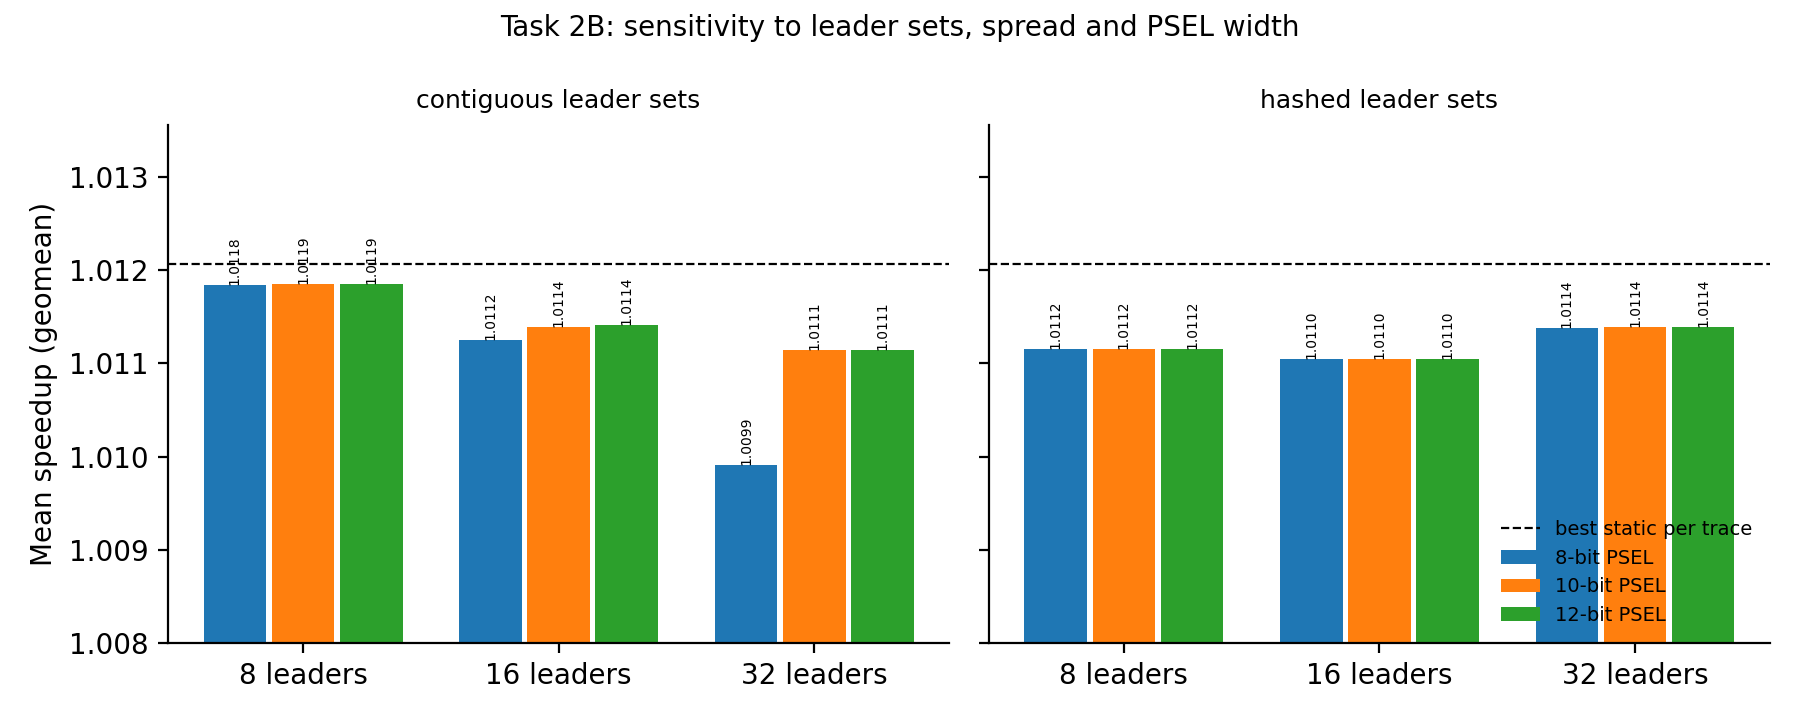
\includegraphics[width=.85\linewidth]{../results/task2b/sensitivity.png}\end{figure}

\textbf{Rationale: number and placement of leader sets.} The leader sets are a sample of the cache, and the selector can only be as good as that sample. Traces 2 and 3 are easy, and almost every configuration picks I-RRIP there. Trace 1 is the hard case. The two modes differ there by only 0.25\%, so the miss counts of the two leader groups are close, and the outcome depends on which sets end up in the sample. With 8 or 16 leaders per policy, the answer depends on placement: contiguous leaders choose SRRIP, while spread leaders choose I-RRIP. When the same number of leaders gives opposite answers, the sample is too small to trust. With 32 spread leaders the choice is SRRIP. With 32 contiguous leaders it flips back and forth (60\% of the time in I-RRIP mode, with 77 switches). Sets $0..63$ are a narrow and unrepresentative slice of the address space, and spreading the leaders over all regions avoids that problem. Eight contiguous leaders had the highest mean (1.0119 against 1.0114), but only because that particular small sample happened to choose correctly on Trace 1. We chose 32 spread leaders because their Trace 1 choice does not depend on luck. The price is that more sets run the losing policy. On Trace 2, the speedup drops from 1.0343 or 1.0346 with 8 leaders to 1.0335 with 32. Going beyond 32 would raise this cost further, with more than 6\% of the cache stuck on the wrong policy, for a choice that is already stable.

\textbf{Rationale: PSEL width.} The width decides how many net misses it takes to change mode. That is half the counter range: 128 for 8 bits, 512 for 10 and 2048 for 12. An 8-bit PSEL is too jumpy. With 32 spread leaders it still spent 2.6\% of Trace 1 follower updates in I-RRIP mode, and with 32 contiguous leaders it switched 87 times on Trace 1 and 25 times on Trace 3, where it cost 0.33\%. At 10 and 12 bits the speedups are identical for every leader configuration. The only difference is that 16 contiguous leaders spend 2.5\% of Trace 1 in I-RRIP mode at 10 bits, with no effect on IPC. So 10 bits is the smallest width at which the decision is stable.

\textbf{Rationale: decision logic.} The selector compares the two policies directly, by the misses they actually cause in their leader sets. It does not try to predict the better policy from the instruction share of accesses, as the ratio formula in the hint does. This matches what the problem asks for (reduce overall misses rather than blindly favour instructions), and there is no threshold to tune, because the decision follows from the measured outcome. Only demand load misses update PSEL, because those are the misses that stall the core. RFO, prefetch and writeback misses are mostly off the critical path, and counting them would push PSEL toward whichever policy reduces traffic rather than stalls. The code also counts instruction and data misses separately for each leader group (printed with the selector statistics), but the decision weights them equally. We did not try other weightings.

\textbf{Storage.} On top of Task 2A's per-line state (2-bit RRPV and the instruction bit, 24576 bits for 1024 sets $\times$ 8 ways), the only addition is the 10-bit PSEL, for 24586 bits in total. Leader identification is combinational logic on the set index. The other counters in the code (follower updates, mode switches, leader misses) are simulation statistics, not part of the design.

\section*{Task 3: SPP with prefetch-aware Dynamic I-RRIP}
\textbf{Policy.} The policy is \texttt{replacement/dyn\_irrip.l2c\_repl} with \texttt{PF\_AWARE} set to 1 (setting it to 0 gives the Task 2B policy). The Task 2B policy is kept as it is, with 32 SRRIP and 32 I-RRIP leader sets and a 10-bit PSEL. Two prefetch rules are added to the I-RRIP mode only, so the SRRIP leader sets still stand for plain SRRIP in the duel. First, a prefetched data line is inserted at RRPV 3, which makes it the first eviction candidate. Second, a prefetch request that hits a line already in the cache does not promote it. Everything else is the Task 2B I-RRIP mode. Instructions are inserted at RRPV 1 and promoted to 0. Demand data is inserted at RRPV 3 and decremented by 1 on a hit, so a prefetched line that is actually used still moves up. Among RRPV-3 lines a data line is evicted first, and data ages by 2. Since the Task 2B I-RRIP mode already inserts all data at RRPV 3, the insertion rule puts prefetches in the same place as demand data. The real prefetch-specific difference is that prefetch hits do not promote.

\textbf{Rationale.} A prefetched line is speculative. Most of the time SPP also fills it into L1D, so the L2 copy only matters if the L1D copy is evicted before it is used. When the L1D MSHR is busy, SPP sends the prefetch to L2 only, and then the L2 copy is the only one. Either way the line has not been used yet, so it should not push out demand data or instruction lines, which are what the L2 is meant to protect. The simulator's L2 statistics support this. With SPP and plain LRU, across the three traces, only 5889 prefetched lines in L2 were later hit by a demand access, while 98282 were evicted unused. A prefetch request that hits in L2 means the L1D prefetcher asked for a line that is in L2 but not in L1D. That is a prediction of future use, not an actual use, so we do not promote on it and leave that to a real demand hit. Inserting at the distant position lets a useless prefetch leave quickly, while a demand hit still rescues a useful one. We swept the prefetch insertion RRPV (1, 2 and 3). RRPV 3 gives the best mean speedup (1.0236, against 1.0223 and 1.0225), and inserting prefetches closer than demand data raises the L2 instruction MPKI (7.25 at RRPV 3, 7.31 at RRPV 1).

\textbf{Results} (25M warmup + 25M simulation instructions, speedup is the geometric mean over the three traces).
\textbf{IPC}\\[2pt]
\begin{tabular}{lrrrr}\toprule
Config & Trace1 & Trace2 & Trace3 & Mean \\ \midrule
Baseline (no pf, LRU) & 0.2323 & 0.2512 & 0.3821 & 0.2885 \\
SPP & 0.2343 & 0.2549 & 0.3872 & 0.2921 \\
Dynamic IRRIP & 0.2323 & 0.2525 & 0.3821 & 0.2889 \\
SPP + Dyn IRRIP (pf-unaware) & 0.2342 & 0.2562 & 0.3874 & 0.2926 \\
SPP + Dyn IRRIP (pf-aware) & 0.2344 & 0.2564 & 0.3875 & 0.2928 \\
PF insert RRPV 1 & 0.2342 & 0.2557 & 0.3872 & 0.2923 \\
PF insert RRPV 2 & 0.2344 & 0.2561 & 0.3874 & 0.2926 \\
PF insert RRPV 3 (final) & 0.2344 & 0.2564 & 0.3875 & 0.2928 \\
\bottomrule\end{tabular}
\medskip

\textbf{Speedup over baseline}\\[2pt]
\begin{tabular}{lrrrr}\toprule
Config & Trace1 & Trace2 & Trace3 & Mean \\ \midrule
Baseline (no pf, LRU) & 1.0000 & 1.0000 & 1.0000 & 1.0000 \\
SPP & 1.0082 & 1.0149 & 1.0135 & 1.0122 \\
Dynamic IRRIP & 0.9997 & 1.0052 & 1.0000 & 1.0017 \\
SPP + Dyn IRRIP (pf-unaware) & 1.0078 & 1.0200 & 1.0139 & 1.0139 \\
SPP + Dyn IRRIP (pf-aware) & 1.0087 & 1.0208 & 1.0143 & 1.0146 \\
PF insert RRPV 1 & 1.0079 & 1.0179 & 1.0134 & 1.0131 \\
PF insert RRPV 2 & 1.0087 & 1.0197 & 1.0140 & 1.0141 \\
PF insert RRPV 3 (final) & 1.0087 & 1.0208 & 1.0143 & 1.0146 \\
\bottomrule\end{tabular}
\medskip

\textbf{L1D load MPKI}\\[2pt]
\begin{tabular}{lrrrr}\toprule
Config & Trace1 & Trace2 & Trace3 & Mean \\ \midrule
Baseline (no pf, LRU) & 10.678 & 13.538 & 3.403 & 9.206 \\
SPP & 9.653 & 12.907 & 3.017 & 8.526 \\
Dynamic IRRIP & 10.678 & 13.538 & 3.403 & 9.207 \\
SPP + Dyn IRRIP (pf-unaware) & 9.657 & 12.906 & 3.017 & 8.526 \\
SPP + Dyn IRRIP (pf-aware) & 9.661 & 12.906 & 3.000 & 8.523 \\
PF insert RRPV 1 & 9.657 & 12.904 & 3.025 & 8.529 \\
PF insert RRPV 2 & 9.656 & 12.904 & 3.014 & 8.525 \\
PF insert RRPV 3 (final) & 9.661 & 12.906 & 3.000 & 8.523 \\
\bottomrule\end{tabular}
\medskip

\textbf{L1D prefetch accuracy (\%)}\\[2pt]
\begin{tabular}{lrrrr}\toprule
Config & Trace1 & Trace2 & Trace3 & Mean \\ \midrule
Baseline (no pf, LRU) & -- & -- & -- & -- \\
SPP & 52.49 & 59.53 & 36.27 & 49.43 \\
Dynamic IRRIP & -- & -- & -- & -- \\
SPP + Dyn IRRIP (pf-unaware) & 52.52 & 59.68 & 36.21 & 49.47 \\
SPP + Dyn IRRIP (pf-aware) & 52.08 & 59.61 & 36.94 & 49.54 \\
PF insert RRPV 1 & 52.03 & 59.68 & 35.92 & 49.21 \\
PF insert RRPV 2 & 52.35 & 59.72 & 36.36 & 49.48 \\
PF insert RRPV 3 (final) & 52.08 & 59.61 & 36.94 & 49.54 \\
\bottomrule\end{tabular}
\medskip

\textbf{L1D load coverage (\%)}\\[2pt]
\begin{tabular}{lrrrr}\toprule
Config & Trace1 & Trace2 & Trace3 & Mean \\ \midrule
Baseline (no pf, LRU) & 0.00 & 0.00 & 0.00 & 0.00 \\
SPP & 9.60 & 4.66 & 11.36 & 8.54 \\
Dynamic IRRIP & 0.00 & -0.00 & 0.00 & -0.00 \\
SPP + Dyn IRRIP (pf-unaware) & 9.57 & 4.67 & 11.36 & 8.53 \\
SPP + Dyn IRRIP (pf-aware) & 9.52 & 4.67 & 11.84 & 8.68 \\
PF insert RRPV 1 & 9.56 & 4.68 & 11.11 & 8.45 \\
PF insert RRPV 2 & 9.57 & 4.68 & 11.45 & 8.57 \\
PF insert RRPV 3 (final) & 9.52 & 4.67 & 11.84 & 8.68 \\
\bottomrule\end{tabular}
\medskip

\textbf{L2C load MPKI}\\[2pt]
\begin{tabular}{lrrrr}\toprule
Config & Trace1 & Trace2 & Trace3 & Mean \\ \midrule
Baseline (no pf, LRU) & 17.696 & 27.357 & 3.954 & 16.336 \\
SPP & 16.880 & 26.784 & 3.456 & 15.707 \\
Dynamic IRRIP & 17.590 & 25.298 & 3.899 & 15.595 \\
SPP + Dyn IRRIP (pf-unaware) & 16.891 & 24.736 & 3.396 & 15.008 \\
SPP + Dyn IRRIP (pf-aware) & 16.749 & 24.609 & 3.359 & 14.906 \\
PF insert RRPV 1 & 16.905 & 25.093 & 3.422 & 15.140 \\
PF insert RRPV 2 & 16.767 & 24.779 & 3.388 & 14.978 \\
PF insert RRPV 3 (final) & 16.749 & 24.609 & 3.359 & 14.906 \\
\bottomrule\end{tabular}
\medskip

\textbf{L2C instruction load MPKI}\\[2pt]
\begin{tabular}{lrrrr}\toprule
Config & Trace1 & Trace2 & Trace3 & Mean \\ \midrule
Baseline (no pf, LRU) & 10.338 & 18.853 & 1.124 & 10.105 \\
SPP & 10.389 & 18.882 & 1.144 & 10.138 \\
Dynamic IRRIP & 10.408 & 17.195 & 1.029 & 9.544 \\
SPP + Dyn IRRIP (pf-unaware) & 10.464 & 17.244 & 1.043 & 9.583 \\
SPP + Dyn IRRIP (pf-aware) & 10.306 & 17.088 & 1.024 & 9.472 \\
PF insert RRPV 1 & 10.475 & 17.677 & 1.055 & 9.736 \\
PF insert RRPV 2 & 10.335 & 17.292 & 1.042 & 9.556 \\
PF insert RRPV 3 (final) & 10.306 & 17.088 & 1.024 & 9.472 \\
\bottomrule\end{tabular}
\medskip

\textbf{L2C data load MPKI}\\[2pt]
\begin{tabular}{lrrrr}\toprule
Config & Trace1 & Trace2 & Trace3 & Mean \\ \midrule
Baseline (no pf, LRU) & 7.358 & 8.504 & 2.830 & 6.231 \\
SPP & 6.491 & 7.903 & 2.312 & 5.569 \\
Dynamic IRRIP & 7.181 & 8.102 & 2.869 & 6.051 \\
SPP + Dyn IRRIP (pf-unaware) & 6.427 & 7.493 & 2.353 & 5.424 \\
SPP + Dyn IRRIP (pf-aware) & 6.443 & 7.522 & 2.335 & 5.433 \\
PF insert RRPV 1 & 6.431 & 7.417 & 2.367 & 5.405 \\
PF insert RRPV 2 & 6.431 & 7.487 & 2.346 & 5.422 \\
PF insert RRPV 3 (final) & 6.443 & 7.522 & 2.335 & 5.433 \\
\bottomrule\end{tabular}
\medskip

\begin{figure}[H]\centering
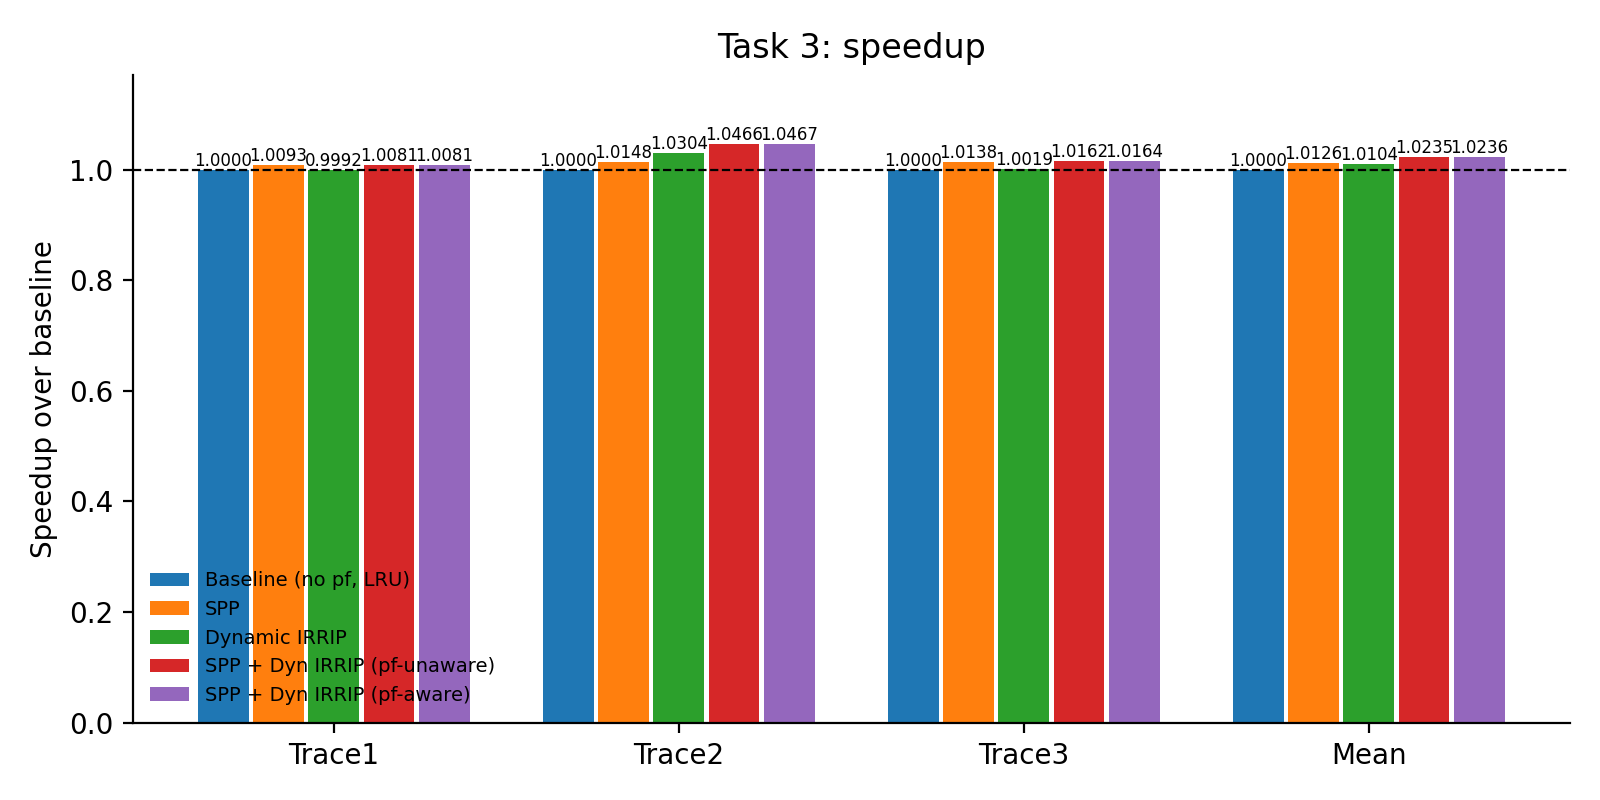
\includegraphics[width=.48\linewidth]{../results/task3/speedup.png}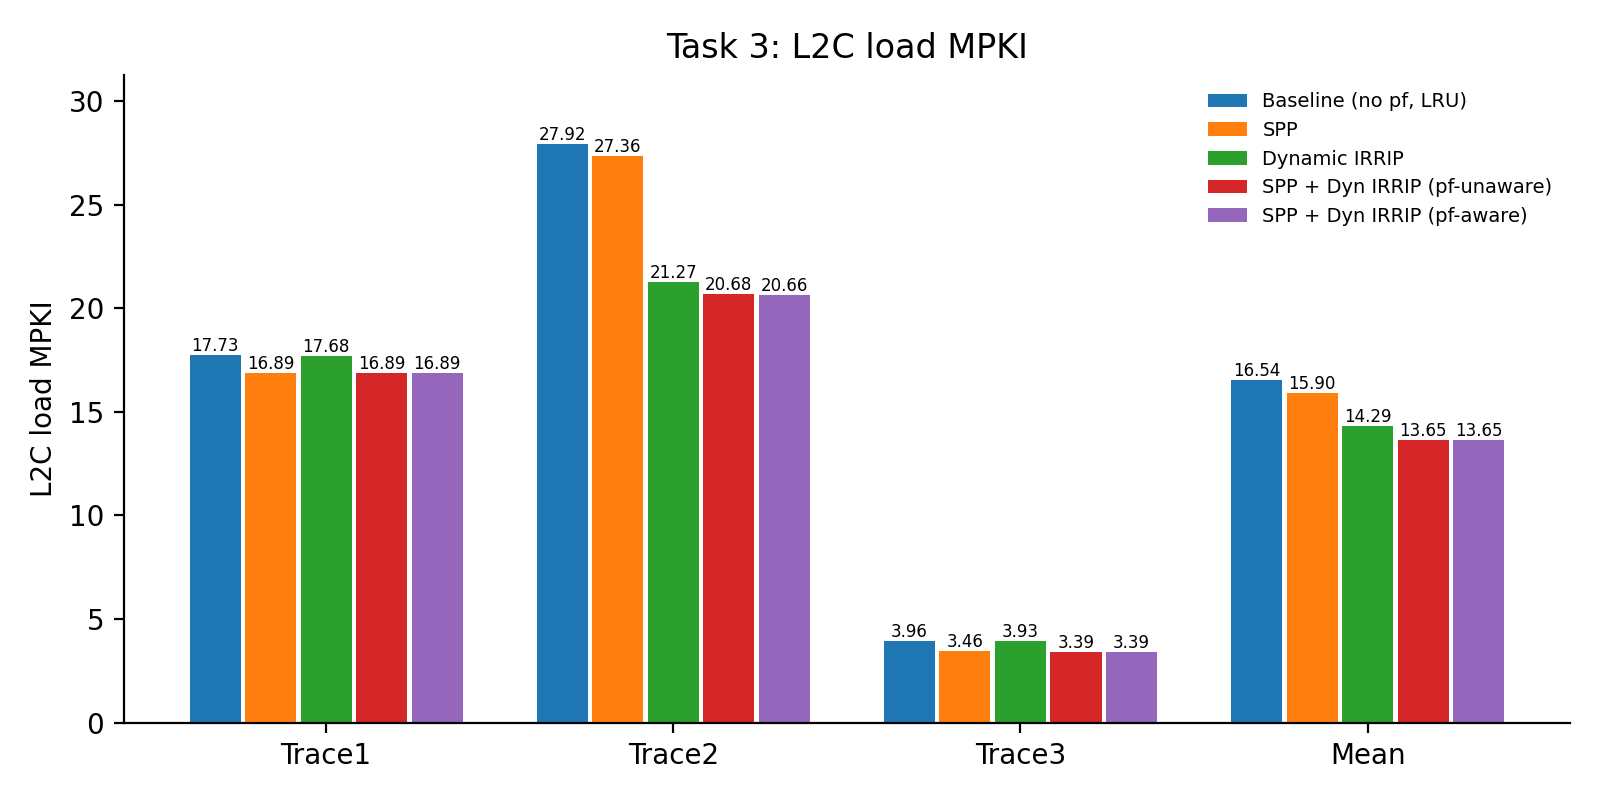
\includegraphics[width=.48\linewidth]{../results/task3/l2_mpki.png}\\
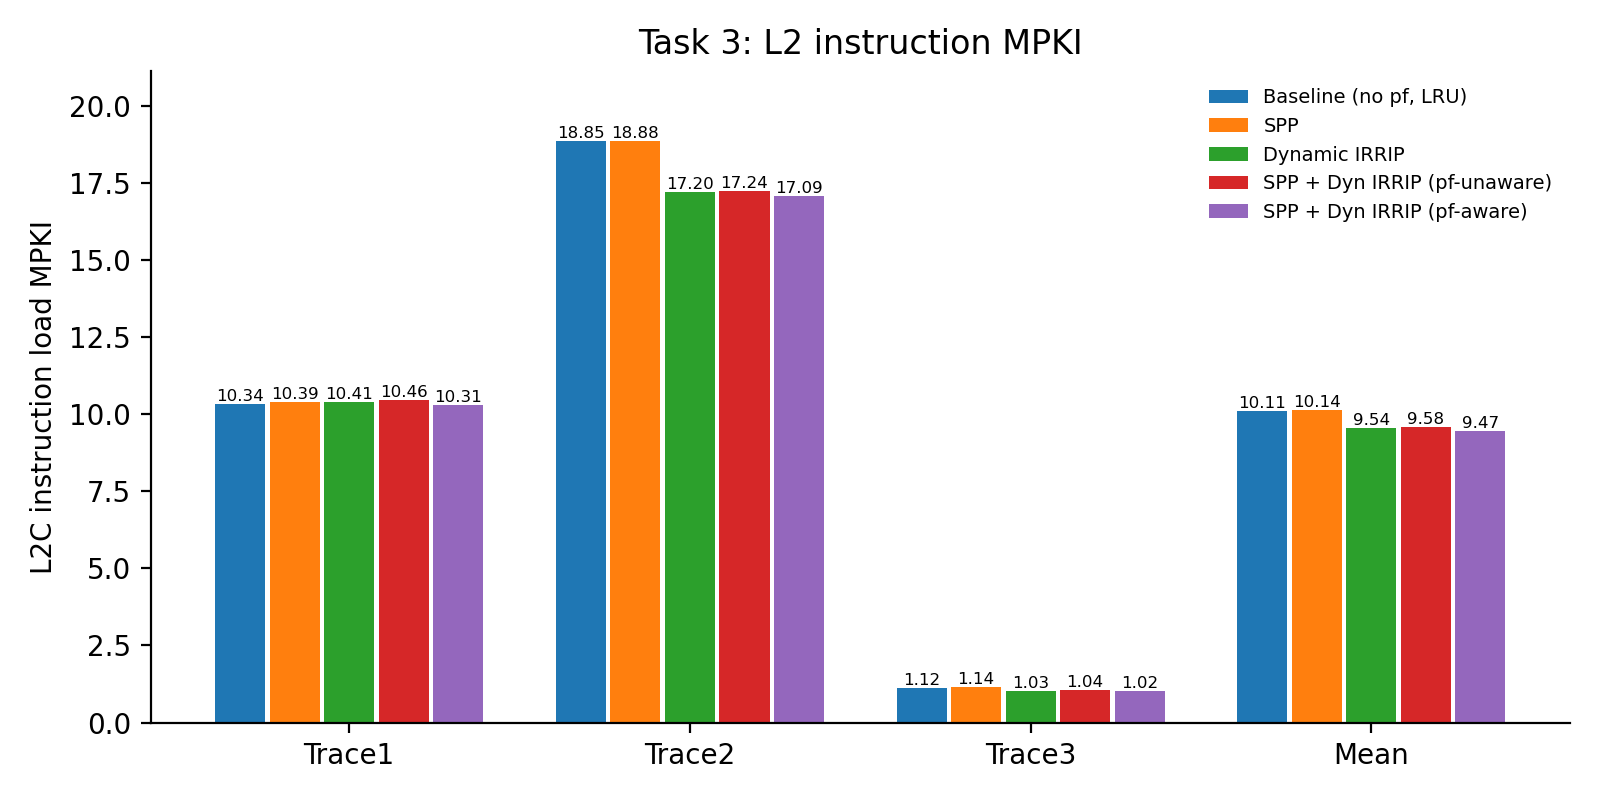
\includegraphics[width=.48\linewidth]{../results/task3/l2_instr_mpki.png}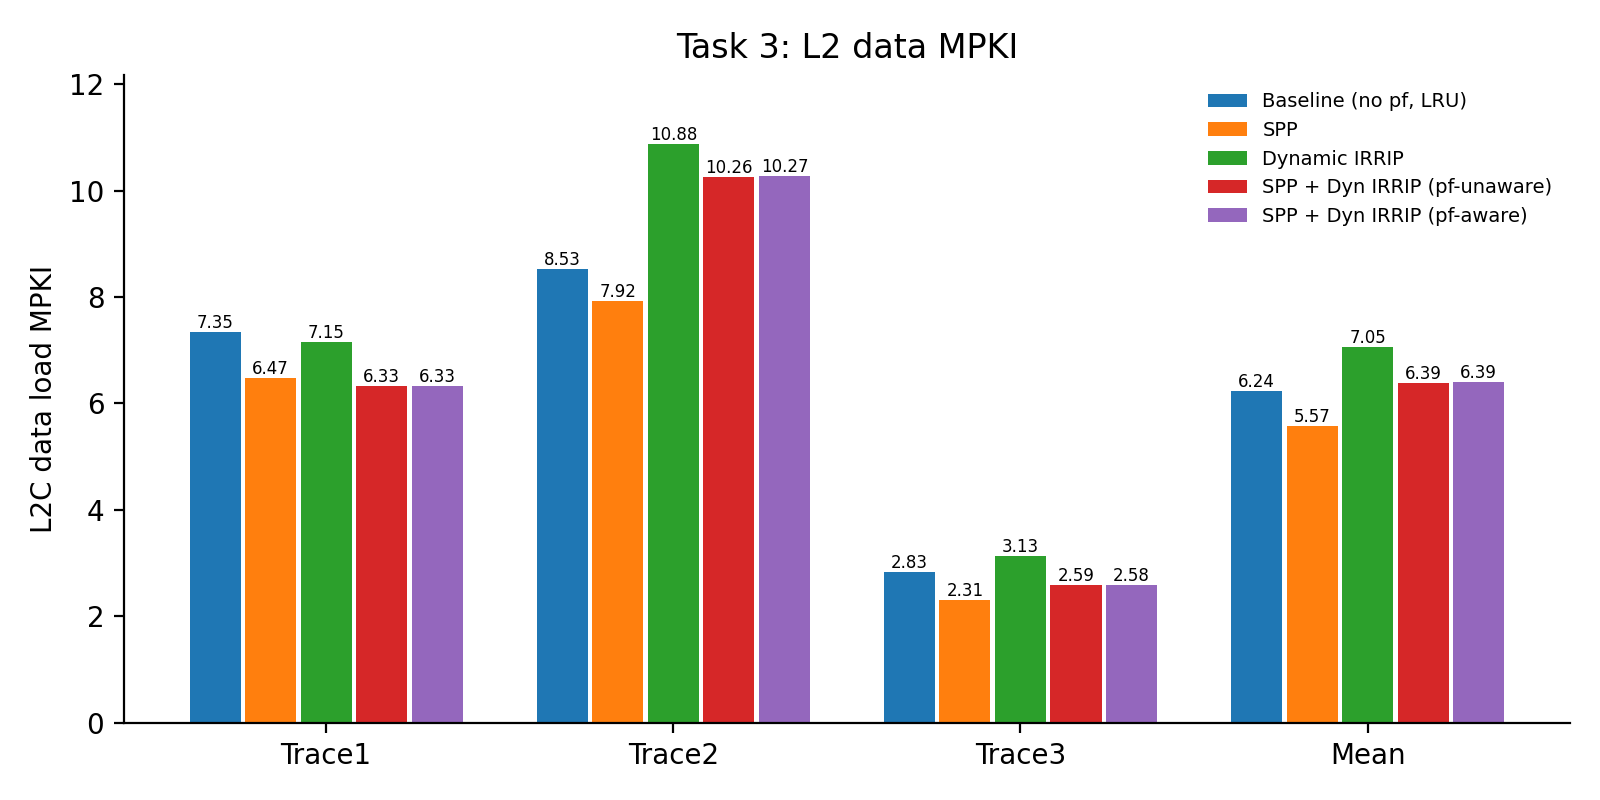
\includegraphics[width=.48\linewidth]{../results/task3/l2_data_mpki.png}\\
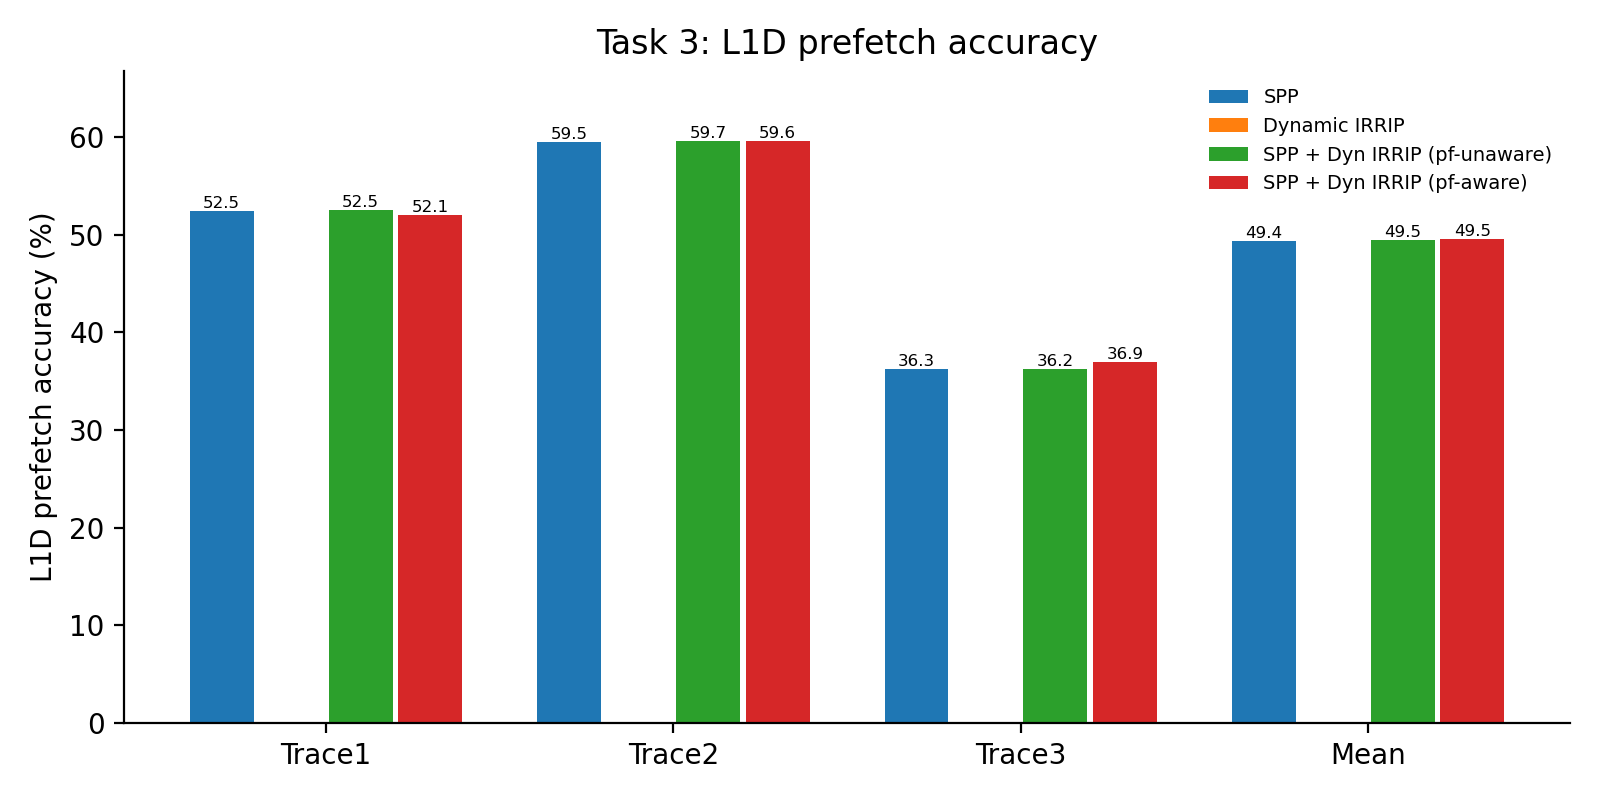
\includegraphics[width=.48\linewidth]{../results/task3/accuracy.png}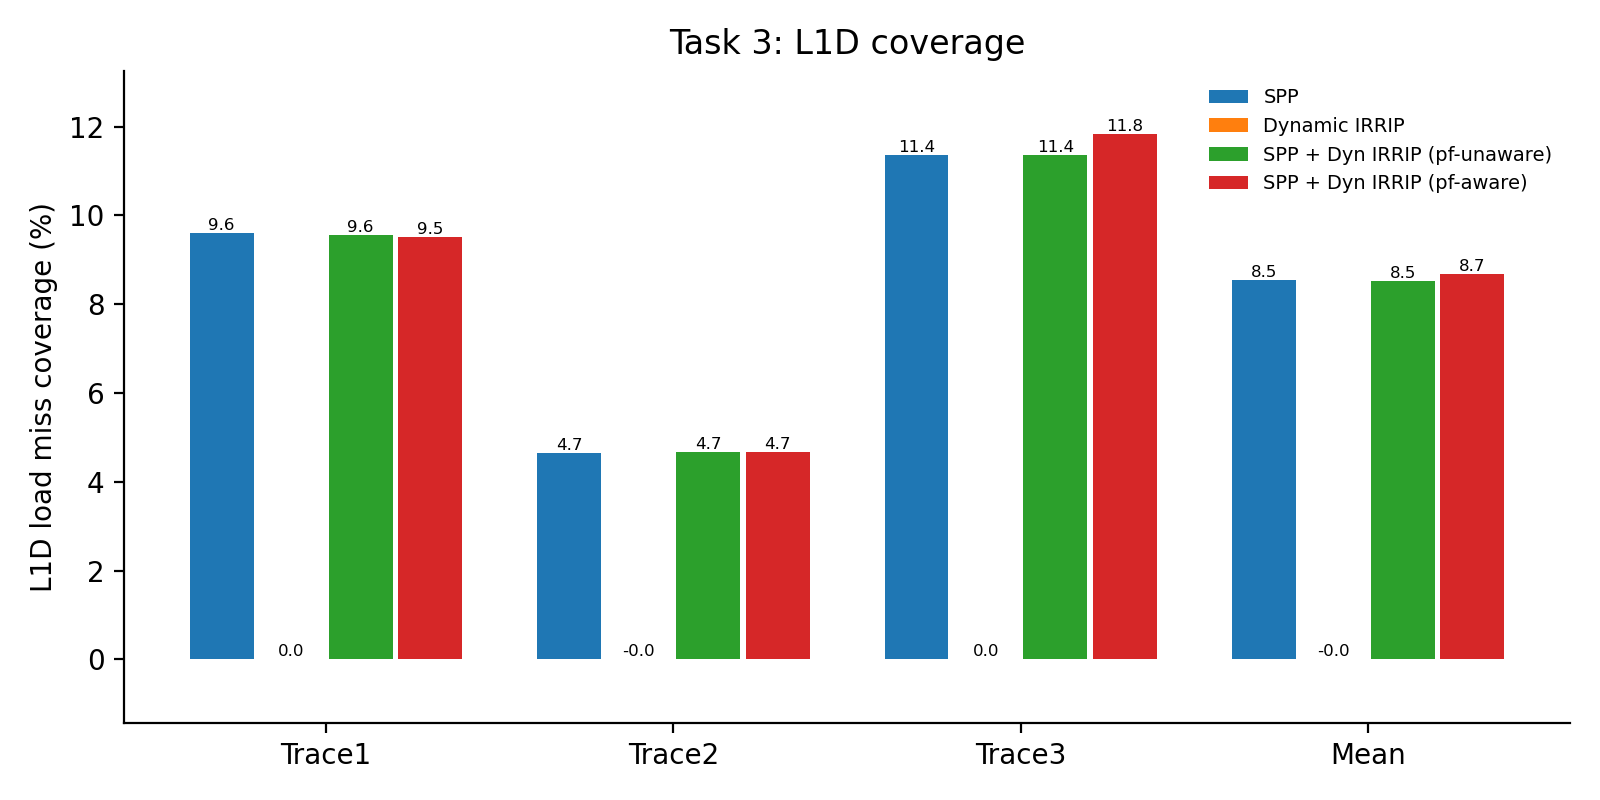
\includegraphics[width=.48\linewidth]{../results/task3/coverage.png}\\
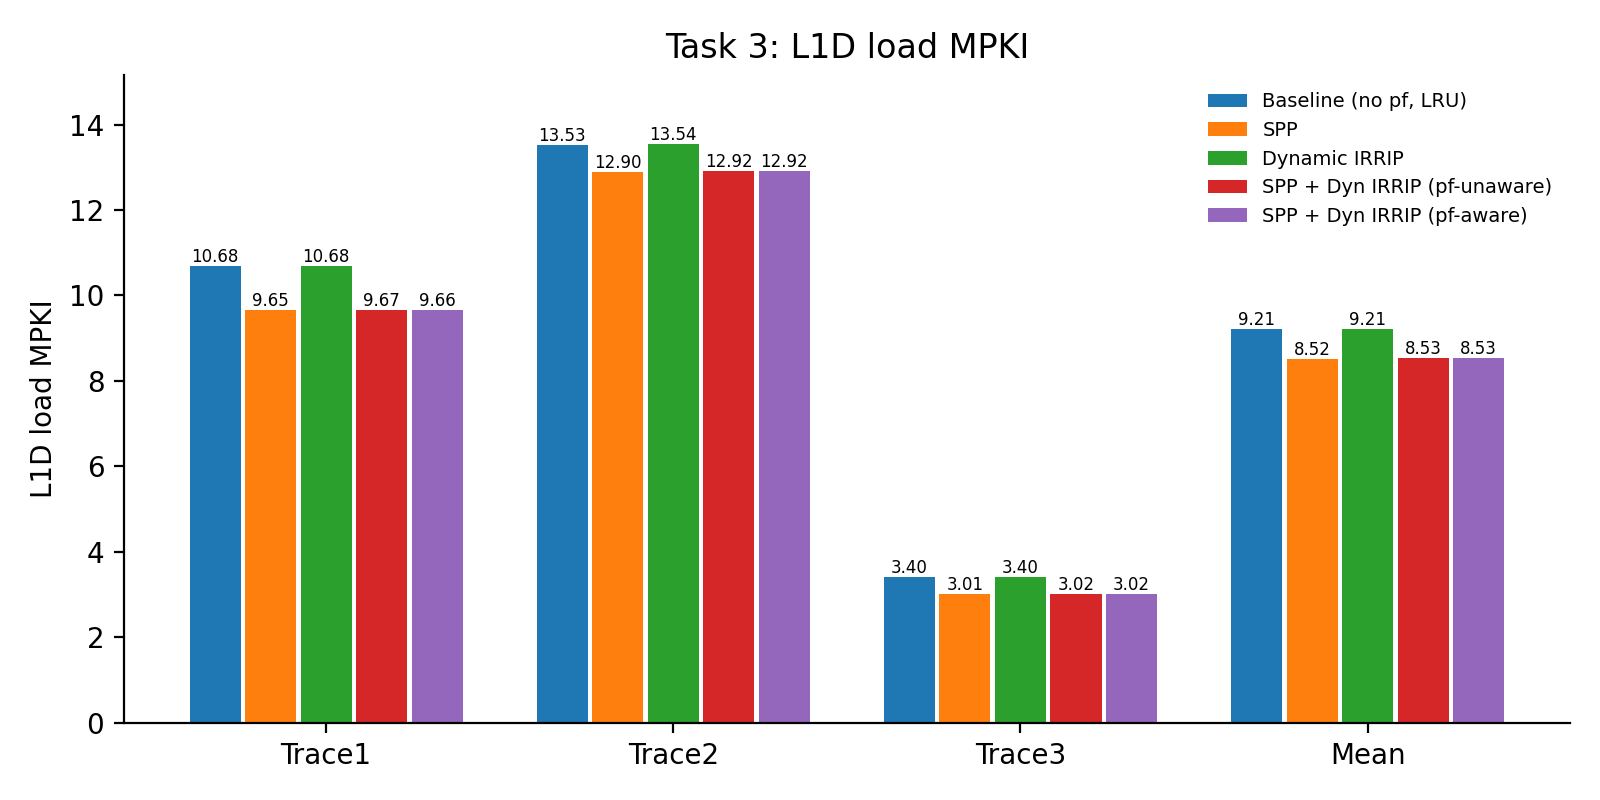
\includegraphics[width=.48\linewidth]{../results/task3/l1d_mpki.png}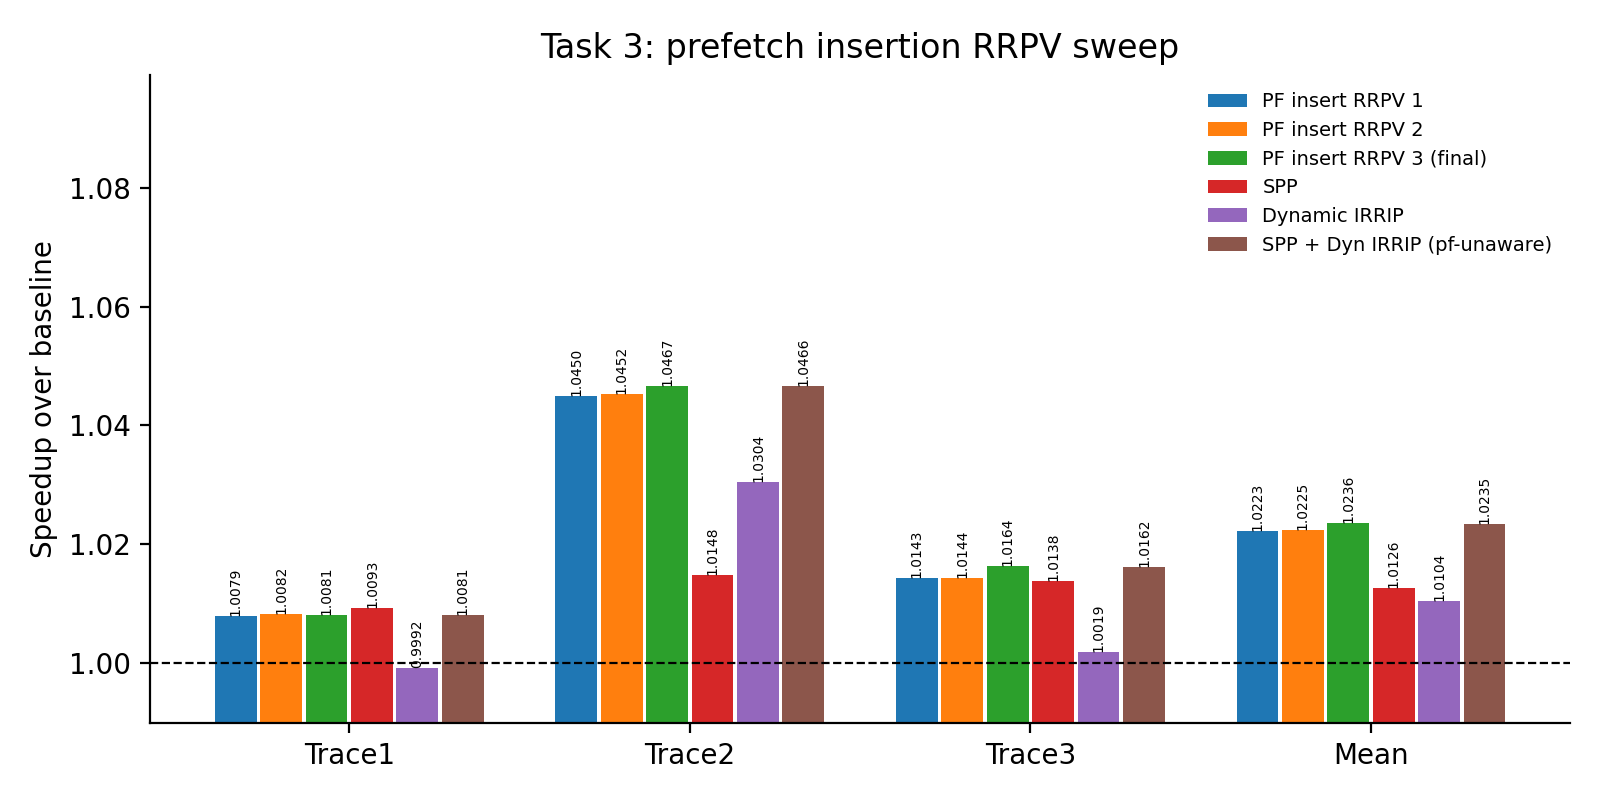
\includegraphics[width=.48\linewidth]{../results/task3/pf_insert_sweep.png}
\end{figure}
\textbf{Findings.} SPP with prefetch-aware Dynamic I-RRIP reaches a mean speedup of 1.0236, against 1.0126 for SPP alone and 1.0104 for Dynamic I-RRIP alone. It beats both on the mean and on Traces 2 and 3 (1.0467 and 1.0164). On Trace 1 it does not beat SPP alone (1.0081 against 1.0093). There the selector picks SRRIP (final PSEL 8 of 1023), so the prefetch rules are only active in the 32 I-RRIP leader sets. The combination also inherits the small Trace 1 loss of Dynamic I-RRIP (0.9992), which comes from the leader sets that keep running I-RRIP. The gain over the prefetch-unaware policy is only 0.0001 in mean speedup, which is within noise for a single 25M-instruction window. With demand data already inserted at RRPV 3, the no-promotion rule is the only thing that separates the two. L2 load MPKI is 13.65 for both (16.54 for the baseline and 15.90 for SPP alone). L1D prefetch accuracy and coverage are essentially unchanged (49.5\% and 8.5\%), because the change affects what stays in L2, not what gets prefetched. Most of the improvement over SPP alone comes from the replacement policy, which brings L2 instruction MPKI down from 10.33 to 7.25.

\section*{Limitations}
Each trace is simulated for one 25M-instruction window. The simulator is deterministic, but differences of around 0.1\% may not carry over to other windows. The SPP accuracy counter does not track prefetches that go only to L2. ChampSim seeds its random number generator from the trace path (\texttt{src/main.cc}), and the seed decides how virtual pages are mapped to physical pages. It adds up the characters of the third-from-last part of the path. The three tasks were run with different path names, so the seed came from \texttt{traces} (the folder name) in Task 1, from \texttt{trace1..3} in Task 2 and from \texttt{Trace1..3} in Task 3. Each task is therefore compared against its own baseline run, and the same configuration can differ slightly between tasks. For example, SPP alone is 1.0122 in Task 1 and 1.0126 in Task 3, and Dynamic I-RRIP is 1.0114 in Task 2B and 1.0104 in Task 3.
\end{document}
